% Template of basic phisics experiment 基于 article template，在此基础上做修改
% 设定文章编码类型，正文字号为五号则 zihao=5，正文字号为小四则 zihao=-4
\documentclass[zihao=5, UTF8]{article}		


% 自定义宏定义
\def\N{\mathbb{N}}
\def\F{\mathbb{F}}
\def\Z{\mathbb{Z}}
\def\Q{\mathbb{Q}}
\def\R{\mathbb{R}}
\def\C{\mathbb{C}}
\def\T{\mathbb{T}}
\def\S{\mathbb{S}}
\def\A{\mathbb{A}}
\def\I{\mathscr{I}}
\def\d{\mathrm{d}}
\def\p{\partial}


% 物理实验报告所需的其它宏包
\usepackage{ulem}   % \uline 下划线支持

% 导入基本宏包
\usepackage[UTF8]{ctex}     % 设置文档为中文语言
\usepackage[colorlinks, linkcolor=blue, anchorcolor=blue, citecolor=blue, urlcolor=blue]{hyperref}  % 宏包：自动生成超链接 (此宏包与标题中的数学环境冲突)
% \usepackage{docmute}    % 宏包：子文件导入时自动去除导言区，用于主/子文件的写作方式，\include{./51单片机笔记}即可。注：启用此宏包会导致.tex文件capacity受限。
\usepackage{amsmath}    % 宏包：数学公式
\usepackage{mathrsfs}   % 宏包：提供更多数学符号
\usepackage{amssymb}    % 宏包：提供更多数学符号
\usepackage{pifont}     % 宏包：提供了特殊符号和字体
\usepackage{extarrows}  % 宏包：更多箭头符号

% 列表环境设置
\usepackage{enumitem}   % 宏包：列表环境设置
    \setlist[enumerate]{itemsep=0pt, parsep=0pt, topsep=0pt, partopsep=0pt, leftmargin=3.5em} 
    \setlist[itemize]{itemsep=0pt, parsep=0pt, topsep=0pt, partopsep=0pt, leftmargin=3.5em}
    \newlist{circledenum}{enumerate}{1} % 创建一个新的枚举环境  
    \setlist[circledenum,1]{  
        label=\protect\circled{\arabic*}, % 使用 \arabic* 来获取当前枚举计数器的值，并用 \circled 包装它  
        ref=\arabic*, % 如果需要引用列表项，这将决定引用格式（这里仍然使用数字）
        itemsep=0pt, parsep=0pt, topsep=0pt, partopsep=0pt, leftmargin=3.5em
    }  
% 文章页面 margin 设置
\usepackage[a4paper]{geometry}  % 宏包：文章页面 margin 设置
    \geometry{top=0.75in}
    \geometry{bottom=0.75in}
    \geometry{left=0.75in}
    \geometry{right=0.75in}   % 设置上下左右页边距
    \geometry{marginparwidth=1.75cm}    % 设置边注距离（注释、标记等）

% 自定义数学环境
\usepackage{amsthm} % 宏包：数学环境配置
% theorem-line 环境自定义
    \newtheoremstyle{MyLineTheoremStyle}% <name>
        {11pt}% <space above>
        {11pt}% <space below>
        {}% <body font> 使用默认正文字体
        {}% <indent amount>
        {\bfseries}% <theorem head font> 设置标题项为加粗
        {：}% <punctuation after theorem head>
        {.5em}% <space after theorem head>
        {\textbf{#1}\thmnumber{#2}\ \ (\,\textbf{#3}\,)}% 设置标题内容顺序
    \theoremstyle{MyLineTheoremStyle} % 应用自定义的定理样式
    \newtheorem{LineTheorem}{Theorem.\,}
% theorem-block 环境自定义
    \newtheoremstyle{MyBlockTheoremStyle}% <name>
        {11pt}% <space above>
        {11pt}% <space below>
        {}% <body font> 使用默认正文字体
        {}% <indent amount>
        {\bfseries}% <theorem head font> 设置标题项为加粗
        {：\\ \indent}% <punctuation after theorem head>
        {.5em}% <space after theorem head>
        {\textbf{#1}\thmnumber{#2}\ \ (\,\textbf{#3}\,)}% 设置标题内容顺序
    \theoremstyle{MyBlockTheoremStyle} % 应用自定义的定理样式
    \newtheorem{BlockTheorem}[LineTheorem]{Theorem.\,} % 使用 LineTheorem 的计数器
% definition 环境自定义
    \newtheoremstyle{MySubsubsectionStyle}% <name>
        {11pt}% <space above>
        {11pt}% <space below>
        {}% <body font> 使用默认正文字体
        {}% <indent amount>
        {\bfseries}% <theorem head font> 设置标题项为加粗
        {：\\ \indent}% <punctuation after theorem head>
        {0pt}% <space after theorem head>
        {\textbf{#3}}% 设置标题内容顺序
    \theoremstyle{MySubsubsectionStyle} % 应用自定义的定理样式
    \newtheorem{definition}{}


% 有色文本框及其设置
\usepackage[dvipsnames,svgnames]{xcolor}    %设置插入的文本框颜色
\usepackage[strict]{changepage}     % 提供一个 adjustwidth 环境
\usepackage{framed}     % 实现方框效果
    \definecolor{graybox_color}{rgb}{0.95,0.95,0.96} % 文本框颜色。修改此行中的 rgb 数值即可改变方框纹颜色，具体颜色的rgb数值可以在网站https://colordrop.io/ 中获得。（截止目前的尝试还没有成功过，感觉单位不一样）（找到喜欢的颜色，点击下方的小眼睛，找到rgb值，复制修改即可）
    \newenvironment{graybox}{%
    \def\FrameCommand{%
    \hspace{1pt}%
    {\color{gray}\small \vrule width 2pt}%
    {\color{graybox_color}\vrule width 4pt}%
    \colorbox{graybox_color}%
    }%
    \MakeFramed{\advance\hsize-\width\FrameRestore}%
    \noindent\hspace{-4.55pt}% disable indenting first paragraph
    \begin{adjustwidth}{}{7pt}%
    \vspace{2pt}\vspace{2pt}%
    }
    {%
    \vspace{2pt}\end{adjustwidth}\endMakeFramed%
    }

% 各级标题自定义设置
\usepackage{titlesec}   
    % section标题自定义设置 
    \titleformat{\section}[hang]{\normalfont\huge\bfseries\centering}{第\,\thesection\,部分}{20pt}{}
    % subsection标题自定义设置 
    \titleformat{\subsection}[hang]{\normalfont\Large\bfseries}{\,\thesubsection\,}{8pt}{}
    % subsubsection标题自定义设置
    \titleformat{\subsubsection}[hang]{\normalfont\large\bfseries}{\,\thesubsubsection\,}{6pt}{}

% 外源代码插入设置
\usepackage{matlab-prettifier}
    \lstset{
        style=Matlab-editor,  % 继承matlab代码颜色等
    }
\usepackage[most]{tcolorbox} % 引入tcolorbox包 
\usepackage{listings} % 引入listings包
    \tcbuselibrary{listings, skins, breakable}
    \lstdefinestyle{matlabstyle}{
        language=Matlab,
        basicstyle=\small,
        breakatwhitespace=false,
        breaklines=true,
        captionpos=b,
        keepspaces=true,
        numbers=left,
        numbersep=15pt,
        showspaces=false,
        showstringspaces=false,
        showtabs=false,
        tabsize=2
    }
    \newtcblisting{matlablisting}{
        arc=0pt,
        top=0pt,
        bottom=0pt,
        left=1mm,
        listing only,
        listing style=matlabstyle,
        breakable,
        colback=white   % 选一个合适的颜色
    }

% table 支持
\usepackage{booktabs}   % 宏包：三线表
\usepackage{tabularray} % 宏包：表格排版
\usepackage{longtable}  % 宏包：长表格
\usepackage{tabularx}  % 宏包：宽表格
\usepackage{multirow}  % 宏包：表格中一格显示多个项目

% figure 设置
\usepackage{graphicx}  % 支持 jpg, png, eps, pdf 图片 
\usepackage{pdfpages}  % 支持插入 pdf 文件
\usepackage{svg}       % 支持 svg 图片
    \svgsetup{
        % 指向 inkscape.exe 的路径
        inkscapeexe = C:/aa_MySame/inkscape/bin/inkscape.exe, 
        % 一定程度上修复导入后图片文字溢出几何图形的问题
        inkscapelatex = false                 
    }


% 图表进阶设置
\usepackage{float}     % 图表位置浮动设置 
\usepackage{caption}    % 图注、表注
    \captionsetup[figure]{name=图}  
    \captionsetup[table]{name=表}
    \captionsetup{labelfont=bf, font=small}

% 文章默认字体设置
    \usepackage{fontspec}   % 宏包：字体设置
       \setmainfont{SimSun}    % 设置中文字体为宋体字体
      \setCJKmainfont[AutoFakeBold=3]{SimSun} % 设置加粗字体为 SimSun 族，AutoFakeBold 可以调整字体粗细^     \setmainfont{Times New Roman} % 设置英文字体为Times New Roman


% 其它设置
    % equation 公式编号设置
        \makeatletter  
        \renewcommand{\theequation}{\thesection.\arabic{equation}}  
        \makeatother
    % 脚注设置
        \renewcommand\thefootnote{\ding{\numexpr171+\value{footnote}}}
    % 参考文献引用设置
        \bibliographystyle{unsrt}   % 设置参考文献引用格式为unsrt
        \newcommand{\upcite}[1]{\textsuperscript{\cite{#1}}}     % 自定义上角标式引用
    % 文章序言设置
        \newcommand{\cnabstractname}{序言}
        \newenvironment{cnabstract}{%
            \par\Large
            \noindent\mbox{}\hfill{\bfseries \cnabstractname}\hfill\mbox{}\par
            \vskip 2.5ex
            }{\par\vskip 2.5ex}


% 页眉页脚设置
\usepackage{fancyhdr}   %宏包：页眉页脚设置
    \pagestyle{fancy}
    \fancyhf{}
    \cfoot{\thepage}
    \renewcommand\headrulewidth{1pt}
    \renewcommand\footrulewidth{0pt}
    \rhead{\bfseries 分组序号: YK04-2}    
    \chead{《基础物理实验》实验报告,\ 韩初晓,\ 2023K8009908002}
    \lhead{2024.10.10}

% 文档信息设置
%\title{这里是标题\\The Title of the Report}
%\author{丁毅\\ \footnotesize 中国科学院大学，北京 100049\\ Yi Ding \\ %\footnotesize University of Chinese Academy of Sciences, Beijing %100049, China}
%\date{\footnotesize 2024.8 -- 2025.1}

% 开始编辑文章

\begin{document}
\noindent\begin{flushright}
    \zihao{2}{分组序号: YK04-2}
\end{flushright}

\setCJKfamilyfont{boldsong}[AutoFakeBold = {2.17}]{SimSun}
\newcommand*{\boldsong}{\CJKfamily{boldsong}}


\begin{center}\large
    \noindent{\Huge\bfseries\boldsong《基础物理实验》实验报告 }
    \\\vspace{0.4cm}
    \noindent\textit{
        \textbf{\boldsong 实验名称：}\uline{\hspace{1.7cm} 磁场的测量\hspace{1.7cm}}\hspace{0.4cm} 
        指导教师：\uline{\hspace{1.0cm}丰家峰\hspace{1.0cm}}}
    \\\vspace{0.1cm}
    \noindent\textit{
        姓名：\uline{\,\,\,韩初晓\,\,\,}\hspace{0.2cm}
        学号：\uline{\,\,\,{\upshape 2023K8009908002}\,\,\,}\hspace{0.2cm}
        专业：\uline{\,\,\,计算机科学与技术\,\,\,}\hspace{0.2cm}
        班级：\uline{\,\,\,\upshape{2306}\,\,\,}}
    \\\vspace{0.1cm}
    \noindent\textit{
        实验日期：\uline{\,\,{\upshape 2024.11.14}\,\,}\hspace{0.2cm}
        实验地点：\uline{\,\,\,教学楼{\upshape708}\,\,\,}\hspace{0.2cm}
        是否调课/补课：\uline{\hspace{0.5cm}否\hspace{0.5cm}}\hspace{0.2cm}
        成绩：\uline{\hspace{2cm}}}
\end{center}
% \vspace{-0.2cm}
\noindent\rule{\textwidth}{0.1em}   % 分割线

% 控制目录不换页
\vspace{1cm}
\setcounter{tocdepth}{2}  % 目录深度为 2（不显示 subsubsection）
\noindent\begin{minipage}{\textwidth}\centering
\tableofcontents\thispagestyle{fancy}   % 显示页码、页眉等   
\end{minipage}  
\newpage

\section{利用霍尔效应试验仪测量磁感应强度}\thispagestyle{fancy} 

\subsection{实验用具}

\subsubsection{霍尔效应试验仪}

\begin{figure}[H]
    \centering
    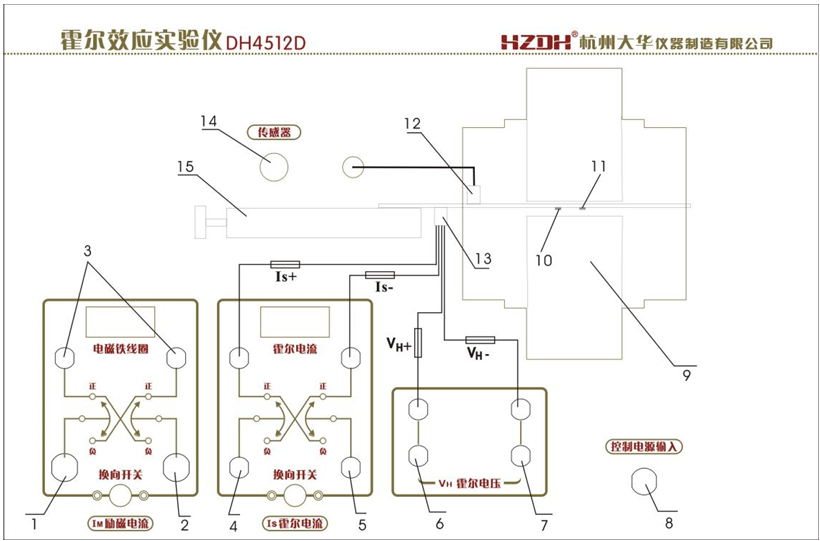
\includegraphics[width=0.6\textwidth]{./hall_effect_apparatus.png}
    \caption{DH4512D霍尔效应实验仪 测试架平面图}
    \label{fig:hall_effect_apparatus}
\end{figure}

\begin{table}[H]
\centering
\begin{tabular}{|c|l|}
\hline
\textbf{编号} & \textbf{功能} \\ \hline
1 & 电磁铁励磁电流 \(I_m\) 输入 A（与测试仪对应 \(I_m\) 输入相连） \\ \hline
2 & 电磁铁励磁电流 \(I_m\) 输入 B（与测试仪对应 \(I_m\) 输入相连） \\ \hline
3 & 电磁铁线圈（内部已连接到电磁铁线圈，无需再连接） \\ \hline
4 & 霍尔工作电流 \(I_s\) 输入 A（与测试仪对应 \(I_s\) 输入相连） \\ \hline
5 & 霍尔工作电流 \(I_s\) 输入 B（与测试仪对应 \(I_s\) 输入相连） \\ \hline
6 & 霍尔电压输出 \(V_H\) +（与测试仪对应 \(V_H\) 输入相连） \\ \hline
7 & 霍尔电压输出 \(V_H\) -（与测试仪对应 \(V_H\) 输入相连） \\ \hline
8 & 控制电源输入（确保电源正常工作，用于打开与关闭仪器） \\ \hline
9 & 探头座（可转换接触方式，用于固定传感器） \\ \hline
10 & 霍尔传感器插座（用于插入霍尔传感器） \\ \hline
11 & 霍尔传感器接头（用于与霍尔传感器相连） \\ \hline
12 & 霍尔传感器连接器（用于将信号传递到仪器检测系统） \\ \hline
13 & 霍尔元件引脚插座（霍尔元件接口，四线输出：\(I_s+\)，\(I_s-\)，\(V_H+\)，\(V_H-\)） \\ \hline
14 & 霍尔传感器插座（与测量仪表相连） \\ \hline
15 & 可移动部件，微调霍尔元件在电磁铁间隙中的位置 \\ \hline
\end{tabular}
\caption{DH4512D 霍尔效应实验仪}
\end{table}

\begin{figure}[H]
    \centering
    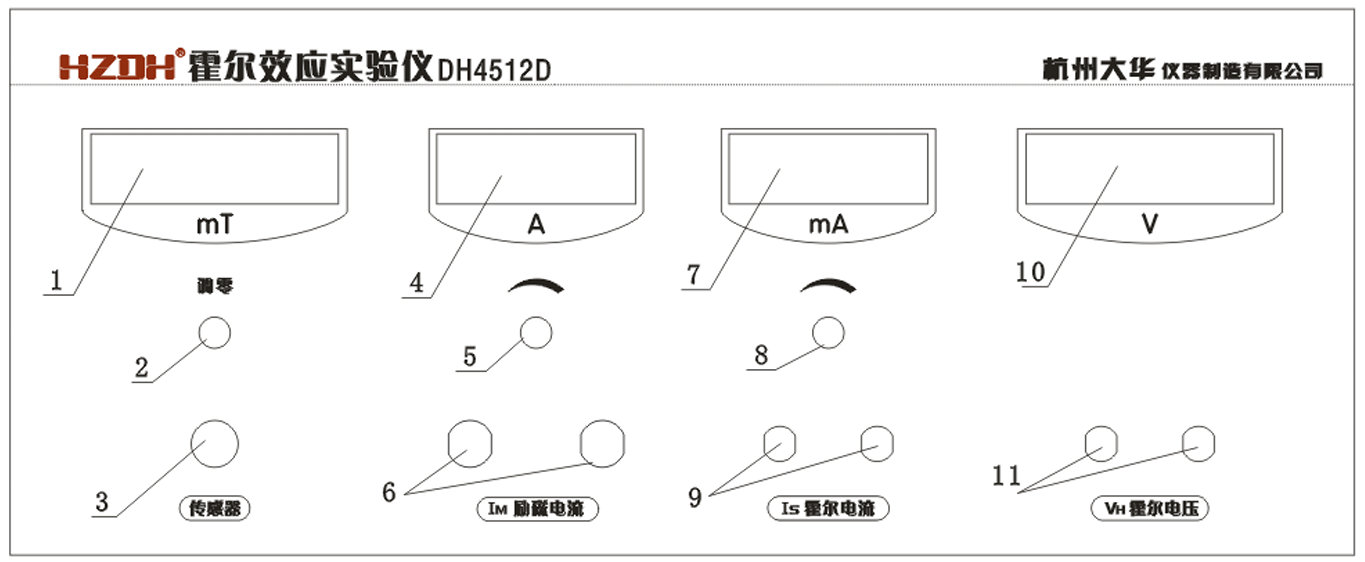
\includegraphics[width=0.6\textwidth]{./hall_effect_apparatus_panel.png}
    \caption{DH4512D霍尔效应实验仪 测试仪面板图}
    \label{fig:hall_effect_apparatus_panel}
\end{figure}

\begin{table}[H]
\centering
\begin{tabular}{|c|l|}
\hline
\textbf{编号} & \textbf{功能} \\ \hline
1 & 霍尔传感器位置显示 \\ \hline
2 & 磁场计调零位置 \\ \hline
3 & 霍尔传感器接口 \\ \hline
4 & \(I_m\) 励磁电流显示 \\ \hline
5 & \(I_m\) 励磁电流调节位置 \\ \hline
6 & \(I_m\) 励磁电流输出接口 \\ \hline
7 & \(I_s\) 霍尔工作电流显示 \\ \hline
8 & \(I_s\) 霍尔工作电流调节位置 \\ \hline
9 & \(I_s\) 霍尔工作电流输出接口 \\ \hline
10 & \(V_H\) 霍尔电压显示 \\ \hline
11 & \(V_H\) 霍尔电压输入接口 \\ \hline
\end{tabular}
\caption{DH4512D 霍尔效应实验仪面板}
\end{table}

\subsection{实验原理}

\subsubsection{霍尔效应}

运动的带电粒子在磁场中受到洛伦兹力作用而发生偏转，导致垂直于电流和磁场方向的两侧电荷积累，从而形成霍尔电场和霍尔电势 $V_H$）。在半导体薄片中，通入工作电流 $I_s$ 时，载流子在磁场 $B$ 的作用下偏转，两侧电荷积累形成的洛伦兹力与反向电场力达到平衡，此时有：

\[
eVB = eE_H = \frac{V_H}{l}
\]

同时，工作电流可表示为：

\[
I_s = neV \cdot l \cdot d
\]

由此推得霍尔电势：

\[
V_H = R_H \cdot I_s \cdot B
\]

其中：

\[
R_H = \frac{1}{ne}
\]

为霍尔系数，反映材料霍尔效应的强弱。定义灵敏度：

\[
K_H = \frac{R_H}{d} = \frac{1}{ned}
\]

则有：

\[
V_H = K_H \cdot I_s \cdot B
\]

灵敏度越高，霍尔元件性能越好。实验中，霍尔元件置于待测磁场中，调整元件平面使磁场垂直（避免角度影响 $V_H = K_H \cdot I_s \cdot B \cdot \cos \theta$），输入恒定工作电流 $I_s$，测量 $V_H$ 即可计算磁感应强度 $B$。

\subsubsection{实验系统误差}

在测量霍尔电势 \( V_H \) 时，由于存在一些副效应，会产生附加电势叠加在 \( V_H \) 上，从而形成测量系统误差。主要副效应及其特点如下：

\begin{enumerate}
    \item \textbf{不等位电势 \( V_0 \)} \\
    由于霍尔片两侧电极焊接不对称、电阻率不均匀或电流端面接触不良（如图4所示），即使未加磁场，A、B两端也可能存在电势差 \( V_0 = I_s R_0 \)。其中 \( R_0 \) 是等位面间的电阻，\( V_0 \) 的大小与 \( I_s \) 成正比，方向随 \( I_s \) 的方向而改变。

    \item \textbf{爱廷豪森效应} \\
    当霍尔片在 \( x \) 方向通以 \( I_s \) 且 \( z \) 方向有磁场 \( B \) 时，载流子的速度分布会导致两侧产生温差（\( T_A - T_B \)），并在不同材料间形成温差电动势 \( V_E \)，满足 \( V_E \propto I_s B \)。该效应与霍尔电势 \( V_H \) 的关系一致，因此无法通过对称测量法消除。

    \item \textbf{伦斯脱效应} \\
    由于控制电流电极的接触电阻不同，会产生焦耳热，导致温差电动势。这种温差电动势引发的热电流在磁场中发生偏转，形成附加电势 \( V_N \propto Q B \)。\( V_N \) 的符号仅随磁场方向变化。

    \item \textbf{里纪-杜勒克效应} \\
    霍尔元件中 \( x \) 方向的温度梯度引发载流子扩散，形成热电流 \( Q \)。在磁场 \( B \) 的作用下，沿 \( y \) 方向产生类似爱廷豪森效应的温差，产生附加电势 \( V_R \propto Q B \)。\( V_R \) 的符号仅与 \( B \) 的方向相关，与 \( I_s \) 无关。
\end{enumerate}

\subsubsection{系统误差的消除方法}

采用对称（交换）测量法消除上述副效应。对四种状态下的测量电势 \( V_{AB} \) 进行组合运算：

\[
V_{AB1} = +V_H + V_0 + V_E + V_N + V_R \quad (\text{当 } +I_s, +I_M)
\]

\[
V_{AB2} = -V_H + V_0 - V_E + V_N + V_R \quad (\text{当 } +I_s, -I_M)
\]

\[
V_{AB3} = +V_H - V_0 + V_E - V_N - V_R \quad (\text{当 } -I_s, -I_M)
\]

\[
V_{AB4} = -V_H - V_0 - V_E - V_N - V_R \quad (\text{当 } -I_s, +I_M)
\]

对以上结果进行如下计算：

\[
\frac{1}{4} \big(V_{AB1} - V_{AB2} + V_{AB3} - V_{AB4}\big) = V_H + V_E
\]

由此可见，除了爱廷豪森效应外的所有副效应均被消除。由于爱廷豪森效应电势 \( V_E \) 的大小在非大电流、非强磁场条件下远小于霍尔电势 \( V_H \)，故 \( V_E \) 可忽略，最终得到：

\[
V_H \approx \frac{1}{4} \big(V_{AB1} - V_{AB2} + V_{AB3} - V_{AB4}\big)
\]


\subsection{实验内容}



\subsection{数据整理和绘图}

\subsubsection{测量霍尔电压 $V_H$ 与工作电流 $I_s$ 的关系}

将霍尔元件移至电磁铁中心，在 $I_M = 0$ 的情况下，调零毫特计；调节 $I_M = 200 \, \text{mA}$，调节 $I_s = 0.5 \, \text{mA}$，按表（1）中 $I_M$ 和 $I_s$ 正负情况切换“测试架”上的电子开关方向，分别测量霍尔电压 $V_H$ 的值（$V_1$, $V_2$, $V_3$, $V_4$），填入表\ref{tab:hall_voltage_current}。以后 $I_s$ 每次递增 $0.50 \, \text{mA}$，测量各 $V_1$, $V_2$, $V_3$, $V_4$ 的值。

根据测量数据，计算每组 $V_1, V_2, V_3, V_4$ 的平均值：

\[
V_H = \frac{V_1 + V_2 + V_3 + V_4}{4}
\]

\begin{table}[H]
\centering
\begin{tabular}{|c|c|c|c|c|c|}
\hline
\multirow{2}{*}{$I_S (mA)$} & \multicolumn{2}{l|}{$+I_M + I_S$} & \multicolumn{2}{l|}{$+I_M - I_S$} & \multicolumn{1}{l|}{$V_H (mV)$} \\ \cline{2-6} 
                             & V1(mV)       & V3(mV)       & V2(mV)       & V4(mV)       &                               \\ \hline
0.00                         & 0.2          & 0.3          & -0.2         & -0.3         & 0.25                          \\ \hline
0.50                         & 23.7         & 28.7         & -23.9        & -28.7        & 26.25                         \\ \hline
1.00                         & 47.5         & 57.5         & -47.8        & -57.6        & 52.6                          \\ \hline
1.50                         & 71.5         & 86.5         & -71.7        & -86.6        & 79.075                        \\ \hline
2.00                         & 94.8         & 115.3        & -95.6        & -115.4       & 105.275                       \\ \hline
2.50                         & 118.6        & 144.6        & -119.6       & -144.2       & 131.75                        \\ \hline
3.00                         & 142.8        & 174.0        & -143.3       & -173.3       & 158.35                        \\ \hline
\end{tabular}
\caption{霍尔电压$V_H$与工作电流$I_S$数据记录}
\label{tab:hall_voltage_current}
\end{table}

将 $V_H$ 平均值与对应的 $I_s$ 作图，绘制 $I_s - V_H$ 曲线。

\begin{figure}[H]
    \centering
    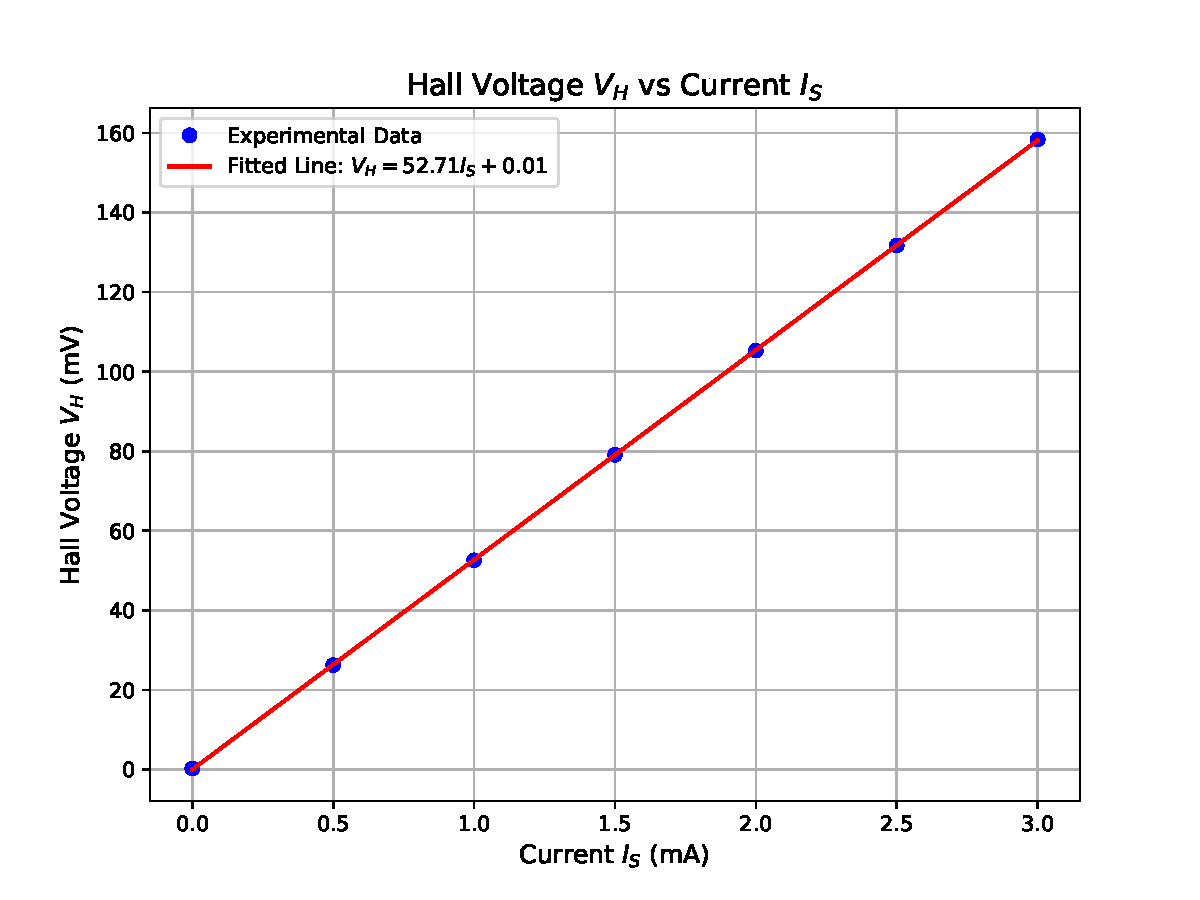
\includegraphics[width=0.6\textwidth]{./hall_voltage_current_1.pdf}
    \caption{霍尔电压$V_H$与工作电流$I_S$关系曲线}
    \label{fig:hall_voltage_current_1}
\end{figure}

根据图片我们可以看出，霍尔电压 $V_H$ 与工作电流 $I_s$ 呈线性关系，且 $V_H = 0$ 时对应 $I_s = 0$，符合理论预期。

\subsubsection{测量霍尔电压 $V_H$ 与励磁电流 $I_M$ 的关系}

1. 将 $I_M$ 和 $I_s$ 调零，调节 $I_s$ 至 $1.00 \, \text{mA}$。

2. 调节 $I_M = 50, 100, 150, \dots, 300 \, \text{mA}$（间隔为 $50 \, \text{mA}$），分别测量霍尔电压 $V_H$ 和磁感应强度 $B$，记录数据到表~\ref{tab:hall_voltage_excitation} 和表~\ref{tab:magnetic_field_excitation}。

3. 根据表~\ref{tab:hall_voltage_excitation} 和表~\ref{tab:magnetic_field_excitation} 中的数据，绘制 $V_H$—$I_M$ 和 $B$—$I_M$ 曲线，进行曲线拟合，验证其线性关系。


\begin{table}[H]
\centering
\begin{tabular}{|c|c|c|c|c|c|}
\hline
\multirow{2}{*}{$I_M (mA)$} & \multicolumn{2}{l|}{$+I_M + I_S$} & \multicolumn{2}{l|}{$+I_M - I_S$} & \multicolumn{1}{l|}{$V_H (mV)$} \\ \cline{2-6} 
                             & V1(mV)       & V3(mV)       & V2(mV)       & V4(mV)       &                               \\ \hline
0.00                         & -4.8         & 4.9          & 4.9          & -4.7         & 4.825                          \\ \hline
50                           & 7.9          & 17.9         & -7.9         & -17.9        & 12.9                           \\ \hline
100                          & 21.2         & 31.2         & -21.2        & -31.2        & 26.2                           \\ \hline
150                          & 34.3         & 44.3         & -34.3        & -44.1        & 39.25                          \\ \hline
200                          & 47.5         & 57.5         & -47.8        & -57.9        & 52.675                         \\ \hline
250                          & 61.1         & 71.4         & -61.4        & -71.3        & 66.3                           \\ \hline
300                          & 73.7         & 83.6         & -73.8        & -83.7        & 78.7                           \\ \hline
\end{tabular}
\caption{霍尔电压$V_H$与励磁电流$I_M$数据记录 ($V_H = \frac{V_1 - V_2 + V_3 - V_4}{4}$)}
\label{tab:hall_voltage_excitation}
\end{table}

\begin{table}[H]
\centering
\begin{tabular}{|c|c|c|c|c|c|}
\hline
\multirow{2}{*}{$B (mT)$} & \multicolumn{2}{l|}{$+I_M + I_S$} & \multicolumn{2}{l|}{$+I_M - I_S$} & \multicolumn{1}{l|}{$V_H (mV)$} \\ \cline{2-6} 
                          & V1(mV)       & V3(mV)       & V2(mV)       & V4(mV)       &                               \\ \hline
0.00                      & -1.4         & -1.4         & -1.3         & -1.4         & 1.375                          \\ \hline
50                        & 35.0         & -17.0        & 35.0         & -17.0        & 26.0                           \\ \hline
100                       & 71.0         & -72.0        & 71.0         & -72.0        & 71.5                           \\ \hline
150                       & 106.6        & -109.2       & 106.6        & -109.2       & 107.9                          \\ \hline
200                       & 141.4        & -143.7       & 141.4        & -143.7       & 142.55                         \\ \hline
250                       & 179.5        & -181.3       & 179.5        & -181.3       & 180.4                          \\ \hline
300                       & 213.5        & -215.0       & 213.6        & -215.4       & 214.375                        \\ \hline
\end{tabular}
\caption{磁感应强度$B$与励磁电流$I_M$数据记录}
\label{tab:magnetic_field_excitation}
\end{table}

4. 利用表~\ref{tab:hall_voltage_excitation} 数据，绘制 $V_H$—$I_M$ 曲线：
   \[
   V_H = k_1 \cdot I_M + b_1
   \]
   其中 $k_1$ 为比例系数，$b_1$ 为截距，通过线性拟合验证 $V_H$ 与 $I_M$ 的线性关系，曲线形貌如下：

\begin{figure}[H]
    \centering
    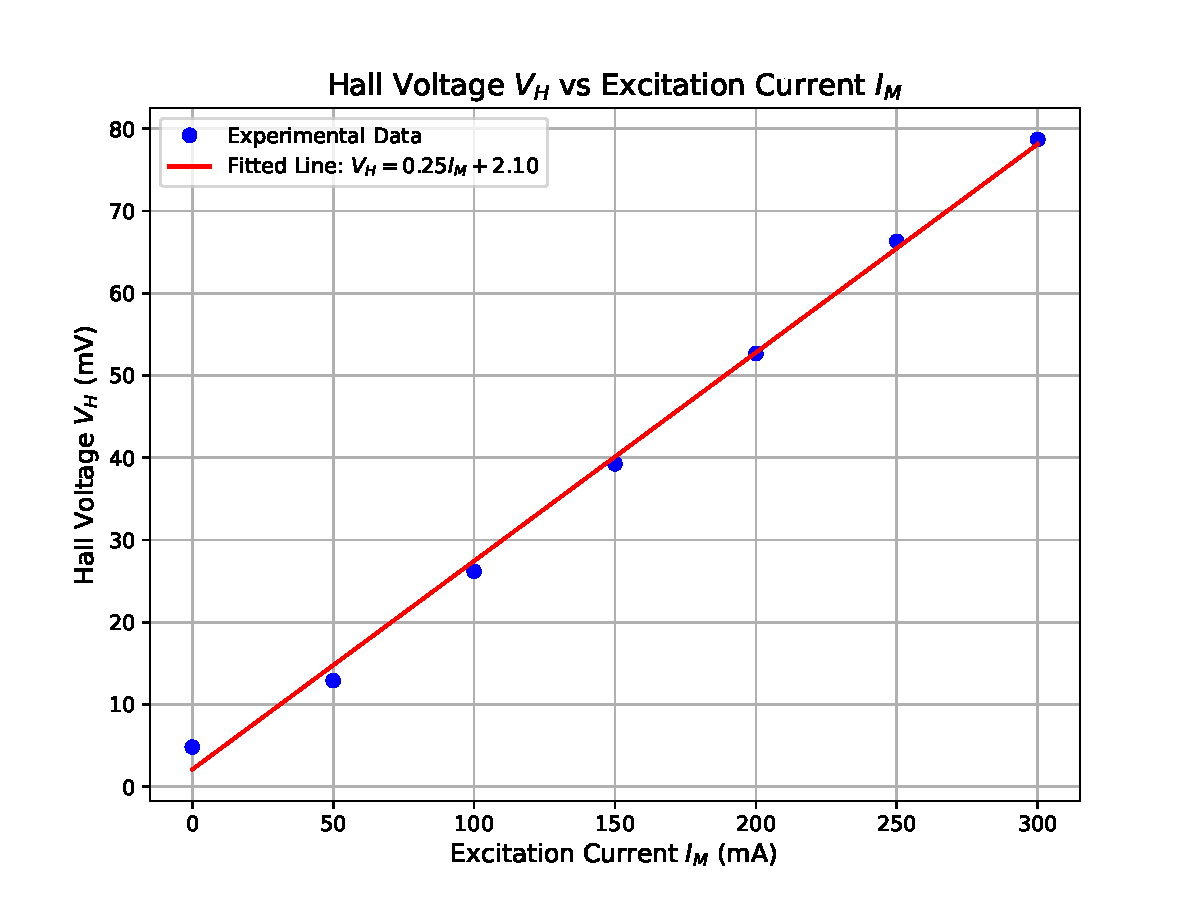
\includegraphics[width=0.6\textwidth]{./hall_voltage_excitation_1.pdf}
    \caption{霍尔电压$V_H$与励磁电流$I_M$关系曲线}
    \label{fig:hall_voltage_excitation_1}
\end{figure}

5. 利用表~\ref{tab:hall_voltage_excitation} 数据，绘制 $B$—$I_M$ 曲线：
   \[
   B = k_2 \cdot I_M + b_2
   \]
   其中 $k_2$ 为比例系数，$b_2$ 为截距，通过线性拟合验证 $B$ 与 $I_M$ 的线性关系。

\begin{figure}[H]
    \centering
    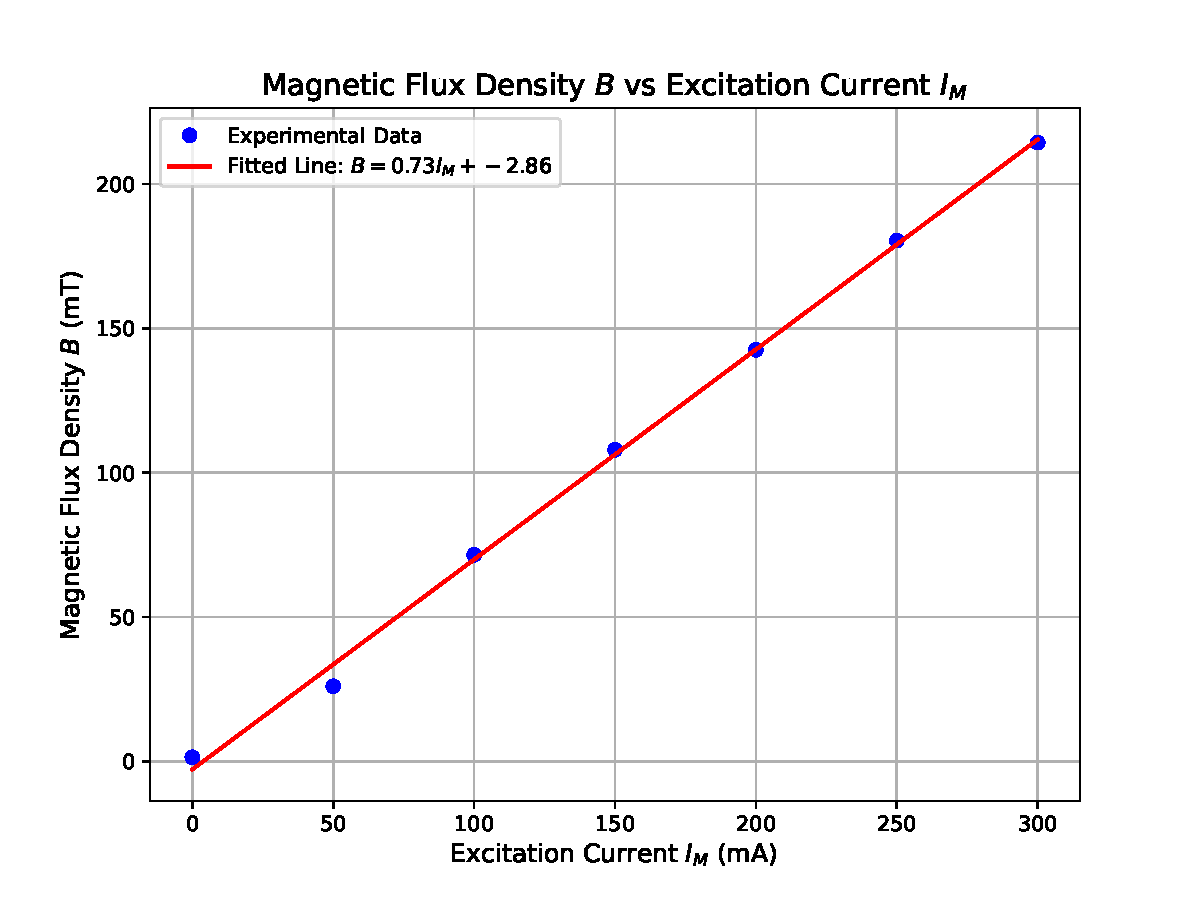
\includegraphics[width=0.6\textwidth]{./magnetic_field_excitation_1.pdf}
    \caption{磁感应强度$B$与励磁电流$I_M$关系曲线}
    \label{fig:magnetic_field_excitation_1}
\end{figure}

\subsubsection{计算霍尔元件的霍尔灵敏度}

如果已知磁感应强度 $B$，根据以下公式可以计算霍尔灵敏度 $K_H$：

\[
K_H = \frac{V_H}{B \cdot I_s}
\]

其中，$K_H$ 表示霍尔灵敏度，$V_H$ 为霍尔电压，$B$ 为磁感应强度，$I_s$ 为工作电流。


根据实验测量的 $V_H$—$B$ 曲线，可以求出曲线斜率 $K_{H-B}$，通过以下公式进一步计算霍尔灵敏度 $K_H$：

\[
K_H = \frac{K_{H-B}}{I_s}
\]

其中，$K_{H-B}$ 是 $V_H$—$B$ 曲线的斜率，$I_s$ 为工作电流。

在实验中，我们已经知道了 $K_{H-I_M}$ 以及 $K_{B-I_M}$ 。可以通过这个值计算出 $K_{H-B}$ 。具体的计算过程见下面公式

\[ K_{H-B} = \frac{K_{H-I_M}}{K_{B-I_M}} = \frac{0.25}{0.73} = 0.342 \]

根据 $$K_H = \frac{K_{H-B}}{I_s}$$ 可以计算出霍尔灵敏度 $K_H$ 的值为 $$K_H = \frac{0.342}{0.001} = 342 \, \text{mV/mA} \cdot \text{T}$$

由此，与标准值 $K_H = 350 \, \text{mV/mA} \cdot \text{T}$ 相比，实验值与标准值误差为 $2.29\%$。



\subsubsection{测量电磁铁磁场沿水平方向分布（选做）}

1. 在 $I_M = 0$ 的情况下，调零毫特计。

2. 调节 $I_M = 200 \, \text{mA}$，并调节移动尺的位置，每隔 $2 \, \text{mm}$ 记录一次毫特计读数，填入表格~\ref{tab:electromagnet_horizontal_distribution}。


\begin{table}[H]
    \centering
    \begin{tabular}{|c|c|c|c|c|c|c|c|}
        \hline
        X/mm & 42 & 40 & 38 & 36 & 34 & 32 & 30 \\ \hline
        B/mT & 45.0 & 87.0 & 136.4 & 142.2 & 143.8 & 143.2 & 143.9 \\ \hline
        X/mm & 28 & 26 & 24 & 22 & 20 & 18 & 16 \\ \hline
        B/mT & 142.7 & 144.0 & 143.9 & 143.2 & 143.8 & 142.8 & 143.9 \\ \hline
    \end{tabular}
    \caption{电磁铁磁场沿水平方向分布数据记录（$I_{M}=200$mA） $I_{S}=0$}
    \label{tab:electromagnet_horizontal_distribution}
\end{table}

根据图表我们可以画出电磁铁磁场沿水平方向分布的图像。

\begin{figure}[H]
    \centering
    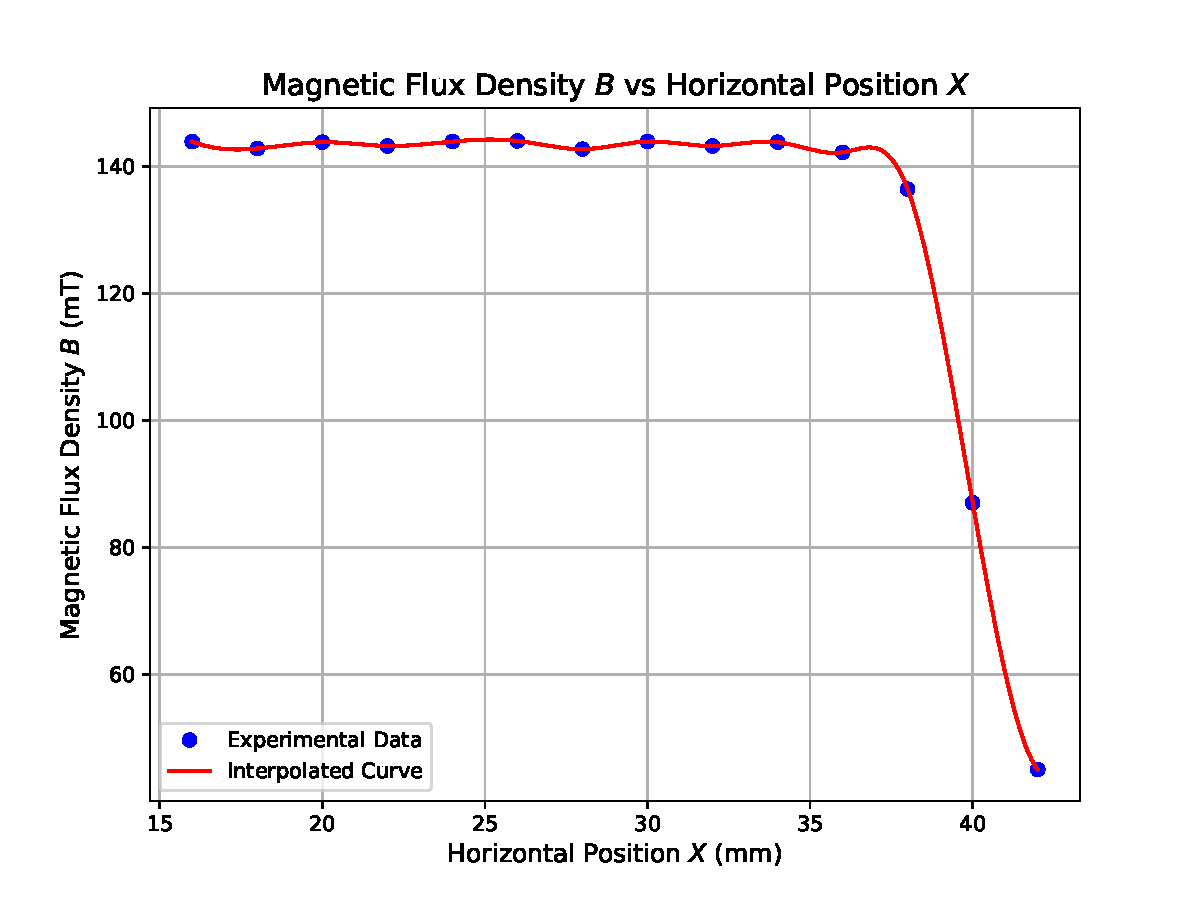
\includegraphics[width=0.6\textwidth]{./electromagnet_horizontal_distribution.pdf}
    \caption{电磁铁磁场沿水平方向分布}
    \label{fig:electromagnet_horizontal_distribution}
\end{figure}

根据图像我们可以看出，电磁铁的磁场在其几何中心附近非常大的区域大致成均匀分布，但在电磁铁的边缘处，随着距离的增加，磁感应强度迅速衰减。这符合理论计算的结果。

\subsubsection{AC模式霍尔效应测量磁场（$I_{S-AC}=1$mA）}


1. 设定 $I_{S-AC} = 1 \, \text{mA}$，并调节励磁电流 $I_M$ 的值。$I_M$ 从 50mA 开始，每次递增 25mA，直到 200mA。

2. 对于每一个设定的 $I_M$ 值，测量对应的磁场强度 $B$（单位：mT）和霍尔电压 $V_{H, AC}$（单位：mV）。将所测得的每个 $I_M$ 值、$B$ 和 $V_{H, AC}$ 填入表格~\ref{tab:ac_hall_effect_measurement}。

3. 根据实验数据，绘制 $I_M$ 与磁场强度 $B$ 的关系图，并绘制 $I_M$ 与霍尔电压 $V_{H, AC}$ 的关系图。根据公式 $K_H = \frac{K_{H-B}}{I_s}$，计算霍尔灵敏度 $K_H$。


\begin{table}[H]
    \centering
    \begin{tabular}{|c|c|c|c|c|c|c|c|}
        \hline
        $I_M$/mA & 50 & 75 & 100 & 125 & 150 & 175 & 200  \\ \hline
        B/mT & 35.6 & 53.5 & 71.1 & 89.4 & 107.2 & 125.1 & 143.2 \\ \hline
        $V_{H, AC}$/mV & 8.804 & 15.228 & 21.790 & 28.428 & 35.087 & 41.938 & 48.162 \\ \hline
    \end{tabular}
    \caption{AC模式霍尔效应测量磁场（$I_{S-AC}=1$mA）}
    \label{tab:ac_hall_effect_measurement}
\end{table}

最终绘制出的图像如下：

\begin{figure}[H]
    \centering
    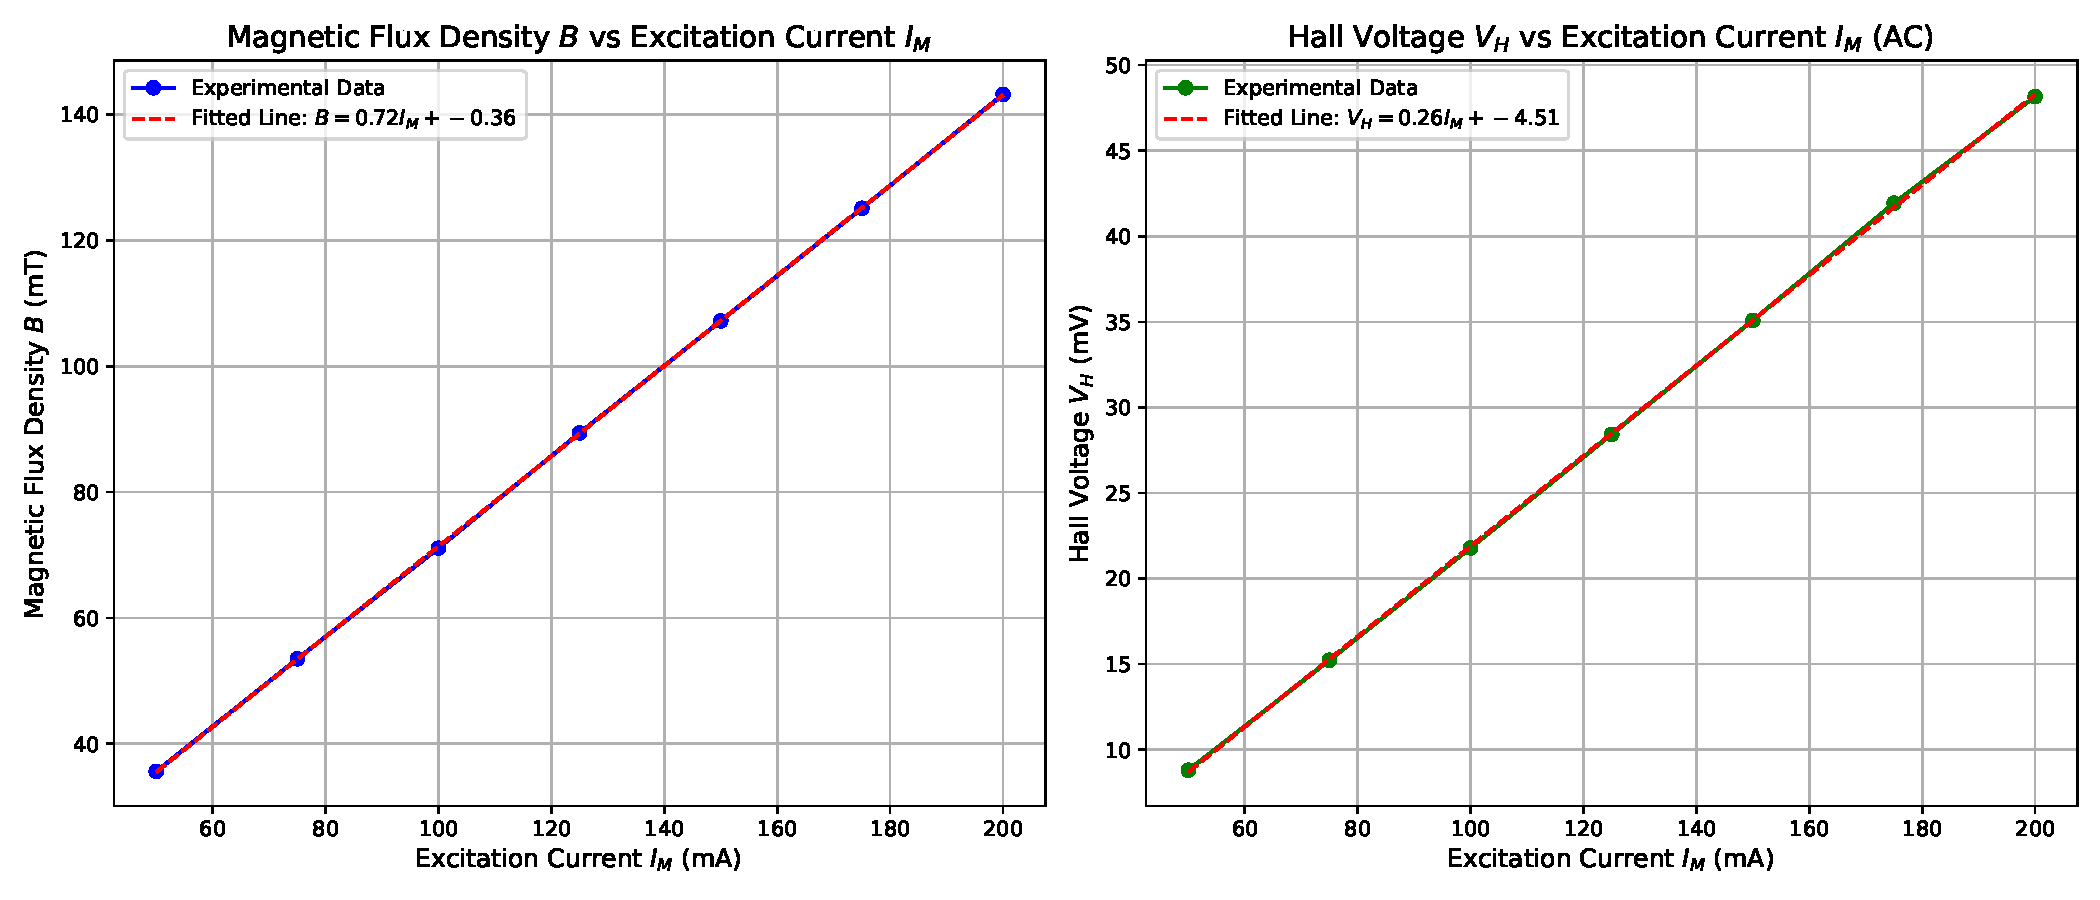
\includegraphics[width=\textwidth]{./ac_hall_effect_measurement.pdf}
    \caption{AC模式霍尔效应测量磁场}
    \label{fig:ac_hall_effect_measurement}
\end{figure}

我们已经知道了 $K_{H-I_M}$ 以及 $K_{B-I_M}$ 。可以通过这个值计算出 $K_{H-B}$ 。具体的计算过程见下面公式

\[ K_{H-B} = \frac{K_{H-I_M}}{K_{B-I_M}} = \frac{0.26}{0.72} = 0.361 \]

根据 $$K_H = \frac{K_{H-B}}{I_s}$$ 可以计算出霍尔灵敏度 $K_H$ 的值为 $$K_H = \frac{0.361}{0.001} = 361 \, \text{mV/mA} \cdot \text{T}$$

由此，与标准值 $K_H = 350 \, \text{mV/mA} \cdot \text{T}$ 相比，实验值与标准值误差为 $3.14\%$。


\section{利用亥姆霍兹线圈测量磁感应强度}

\subsection{实验用具}

\begin{figure}[H]
    \centering
    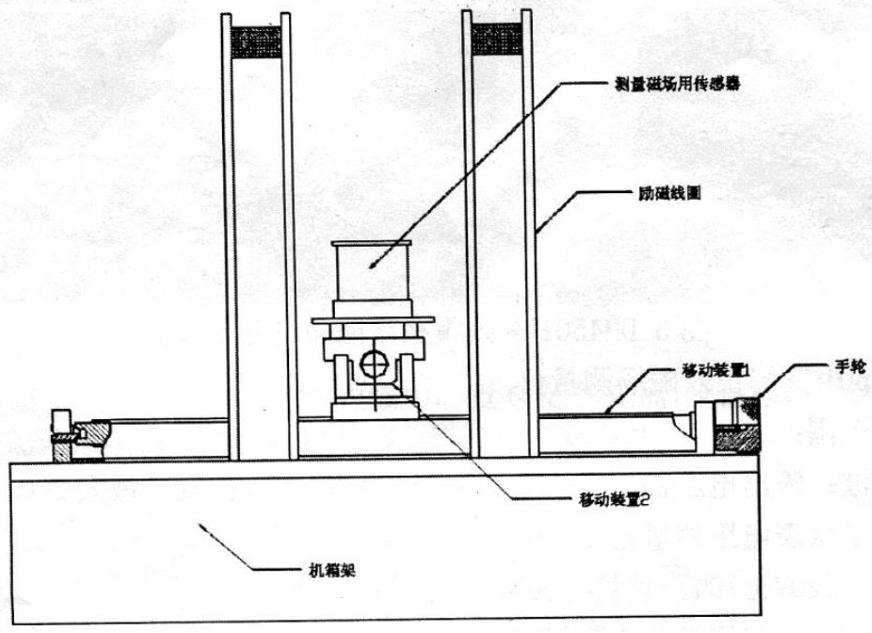
\includegraphics[width=0.6\textwidth]{./helmholtz_coil_apparatus.png}
    \caption{亥姆霍兹线圈架部分}
    \label{fig:helmholtz_coil_apparatus}
\end{figure}

\begin{figure}[H]
    \centering
    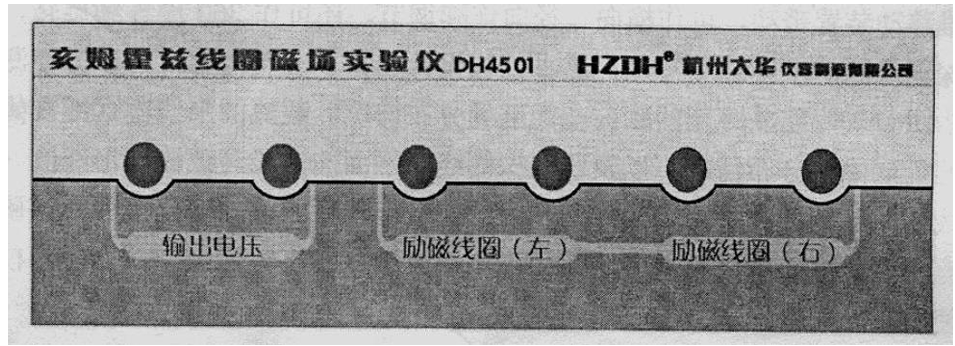
\includegraphics[width=0.6\textwidth]{./helmholtz_coil_apparatus_panel.png}
    \caption{DH4501 亥姆霍兹线圈架面板}
    \label{fig:helmholtz_coil_apparatus_panel}
\end{figure}

\begin{figure}[H]
    \centering
    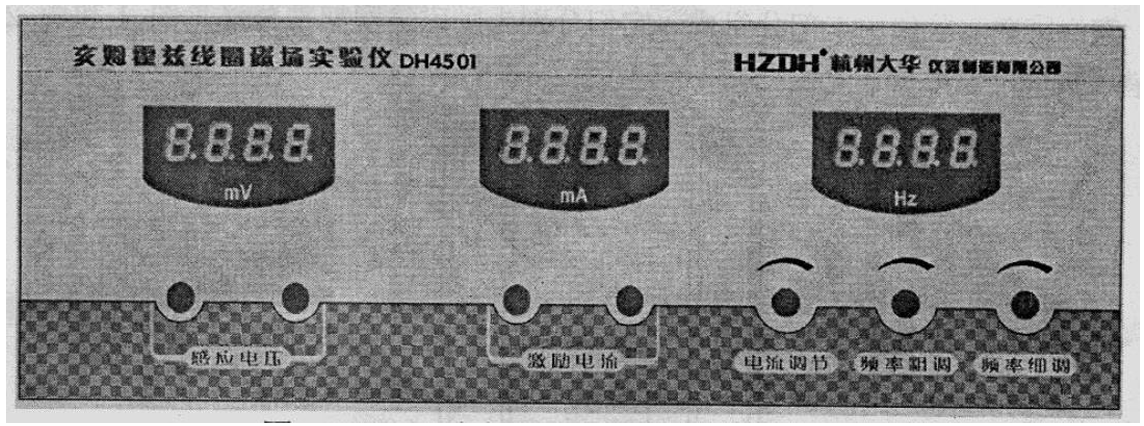
\includegraphics[width=0.6\textwidth]{./helmholtz_coil_apparatus_panel_2.png}
    \caption{DH4501 亥姆霍兹线圈磁感应强度测量仪面板}
    \label{fig:helmholtz_coil_apparatus_panel_2}
\end{figure}

\begin{table}[H]
\centering
\begin{tabular}{|c|l|}
\hline
\textbf{项目} & \textbf{技术参数} \\ \hline
1.1 & \textbf{亥姆霍兹磁线圈架} \\ \hline
& \quad - 线圈有效半径：105 mm \\ \hline
& \quad - 单个线圈匝数：400 匝 \\ \hline
& \quad - 二线圈中心间距：105 mm \\ \hline
& \quad - 移动装置：轴向可移动距离 250 mm，径向可移动距离 70 mm \\ \hline
& \quad - 距离分辨率：1 mm \\ \hline
& \quad - 探测线圈：匝数 1000，旋转角度 360 度 \\ \hline
1.2 & \textbf{磁感应强度测量仪} \\ \hline
& \quad - 频率范围：20 - 200 Hz，频率分辨率：0.1 Hz，测量误差：0.1\% \\ \hline
& \quad - 正弦波：输出电压幅度：最大 20 V\textsubscript{p-p}，输出电流幅度：最大 200 mA \\ \hline
& \quad - 数显毫伏表电压测量范围：0 - 20 mV，测量误差：1\% \\ \hline
1.3 & \textbf{电源} \\ \hline
& \quad - 220 V ± 10\% \\ \hline
1.4 & \textbf{外形尺寸} \\ \hline
& \quad - 亥姆霍兹磁线圈架：340 mm × 270 mm × 250 mm \\ \hline
& \quad - 磁感应强度测量试仪：320 mm × 300 mm × 120 mm \\ \hline
\end{tabular}
\caption{DH4501 亥姆霍兹磁线圈磁感应强度测量仪器}
\end{table}

\subsection{实验原理}

\subsubsection{载流圆线圈的磁感应强度}

对于半径 $ R $、匝数 $ N_0 $、电流 $ I $ 的圆线圈，轴线上距圆心 $ x $ 处的磁感应强度为：
$$
B = \frac{\mu_0 N_0 I R^2}{2(R^2 + x^2)^{3/2}}
$$
其中，$ \mu_0 = 4\pi \times 10^{-7} \, \text{H/m} $。在圆心 $ O $ ($ x = 0 $) 处，磁感应强度计算为：
$$
B = \frac{\mu_0 N_0 I}{2R}
$$

\begin{figure}[H]
    \centering
    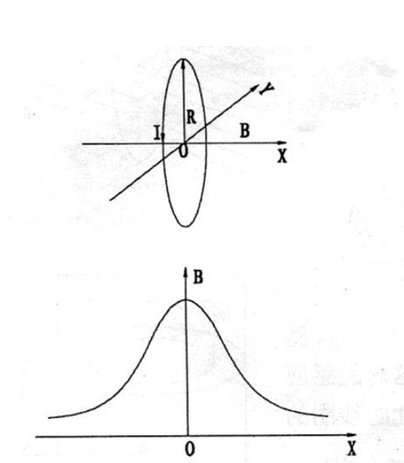
\includegraphics[width=0.6\textwidth]{./single_coil.png}
    \caption{单个圆环线圈的磁感应强度分布示意图}
    \label{fig:single_coil}
\end{figure}

\subsubsection{亥姆霍兹线圈的磁感应强度}

亥姆霍兹线圈由两个相同的圆线圈组成，线圈间距 $ R $。轴线上某点 $ z $ 处的磁感应强度为：
$$
B = \frac{\mu_0 N_0 I R^2}{2} \left[ \left( R^2 + \left( \frac{R}{2} + z \right)^2 \right)^{-3/2} + \left( R^2 + \left( \frac{R}{2} - z \right)^2 \right)^{-3/2} \right]
$$
在中心点 $ O $ ($ z = 0 $) 处，磁感应强度为：
$$
B = \frac{\mu_0 N_0 I}{2R} \times \frac{16}{5^{3/2}}
$$
\begin{figure}[H]
    \centering
    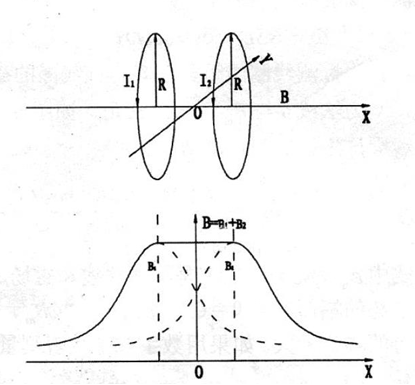
\includegraphics[width=0.6\textwidth]{./helmholtz_coil.png}
    \caption{亥姆霍兹线圈的磁感应强度分布示意图}
    \label{fig:helmholtz_coil}
\end{figure}

\subsubsection{电磁感应法测磁感应强度}


由交流信号驱动线圈产生交变磁场，磁感应强度瞬时值为：
$$
B = B_m \sin \omega t
$$
探测线圈产生的感应电动势为：
$$
e = -\frac{d\Phi}{dt} = NS \omega B_m \cos \theta \cos \omega t
$$
其中，$ e_m = NS \omega B_m \cos \theta $ 是感应电动势的幅值。当 $ \theta = 0 $ 时，$ e_m = NS \omega B_m $，对应有效值为：
$$
B_m = \frac{\sqrt{2} U_{\text{max}}}{NS \omega}
$$
$ B $ 为有效值，与 $ B_m $ 的关系为：
$$
B = \frac{B_m}{\sqrt{2}}
$$
探测线圈的等效面积 $ S $ 计算公式为：
$$
S = \frac{13}{108} \pi D^2
$$
实验中，探测线圈参数为 $ D = 0.012 \, \text{m} $，$ N = 800 $ 匝。例如，交流毫伏表读数 $ U_{\text{max}} = 5.95 \, \text{mV} $ 时，计算得：
$$
B = 0.145 \, \text{mT}
$$


\subsection{实验内容}

\subsection{数据整理和绘图}

\subsubsection{圆电流线圈轴线上磁感应强度的分布测量}

将实验设备连接完成，调节频率调节电位器使频率表显示 120 Hz，调节磁感应强度实验仪的电流调节电位器使励磁电流有效值为 60 mA，以圆电流线圈中心为坐标原点，每隔 5 mm 测量一个 $ U_{\text{max}} $ 值，测量过程中保持励磁电流值不变，探测线圈法线与圆电流线圈轴线夹角为 0°，正反方向测量误差不大于 2\% 时使用一个方向数据，否则取平均值，最终将数据记录于表\ref{tab:circular_current_loop_axis_magnetic_field_distribution}中。

\begin{table}[H] 
    \centering
    \renewcommand{\arraystretch}{1.2} % 增加行距以改善可读性
    \begin{tabular}{|>{\centering\arraybackslash}p{2.5cm}|>{\centering\arraybackslash}p{1cm}|>{\centering\arraybackslash}p{1cm}|>{\centering\arraybackslash}p{1cm}|>{\centering\arraybackslash}p{1cm}|>{\centering\arraybackslash}p{1cm}|>{\centering\arraybackslash}p{1cm}|>{\centering\arraybackslash}p{1cm}|>{\centering\arraybackslash}p{1cm}|>{\centering\arraybackslash}p{1cm}|>{\centering\arraybackslash}p{1cm}|>{\centering\arraybackslash}p{1cm}|}
        \hline
        轴向距离 X/(mm) & -25 & -20 & -15 & -10 & -5 & 0 & 5 & 10 & 15 & 20 & 25 \\ \hline
        $U_{max}$/mV & 5.39 & 5.58 & 5.76 & 5.89 & 5.97 & 6.04 & 6.06 & 6.03 & 5.95 & 5.84 & 5.7 \\ \hline
        测量值 B/(mT) & 0.1314 & 0.1361 & 0.1404 & 0.1436 & 0.1456 & 0.1473 & 0.1478 & 0.1470 & 0.1451 & 0.1424 & 0.1390 \\ \hline
        计算值 B/(mT) & 0.1321 & 0.1361 & 0.1393 & 0.1416 & 0.1431 & 0.1435 & 0.1431 & 0.1416 & 0.1393 & 0.1361 & 0.1321 \\ \hline
        参数 & f & I & $N_0$ & R & & & & & & & \\ \hline
        值 & 120Hz & 60mA & 400 & 105mm & & & & & & & \\ \hline
    \end{tabular}
    \caption{圆电流线圈轴线上磁场分布测量数据记录}
    \label{tab:circular_current_loop_axis_magnetic_field_distribution}
\end{table}

根据表\ref{tab:circular_current_loop_axis_magnetic_field_distribution}中的数据绘制磁感应强度分布曲线，如图\ref{fig:circular_current_loop_axis_magnetic_field_distribution}所示。

\begin{figure}[H]
    \centering
    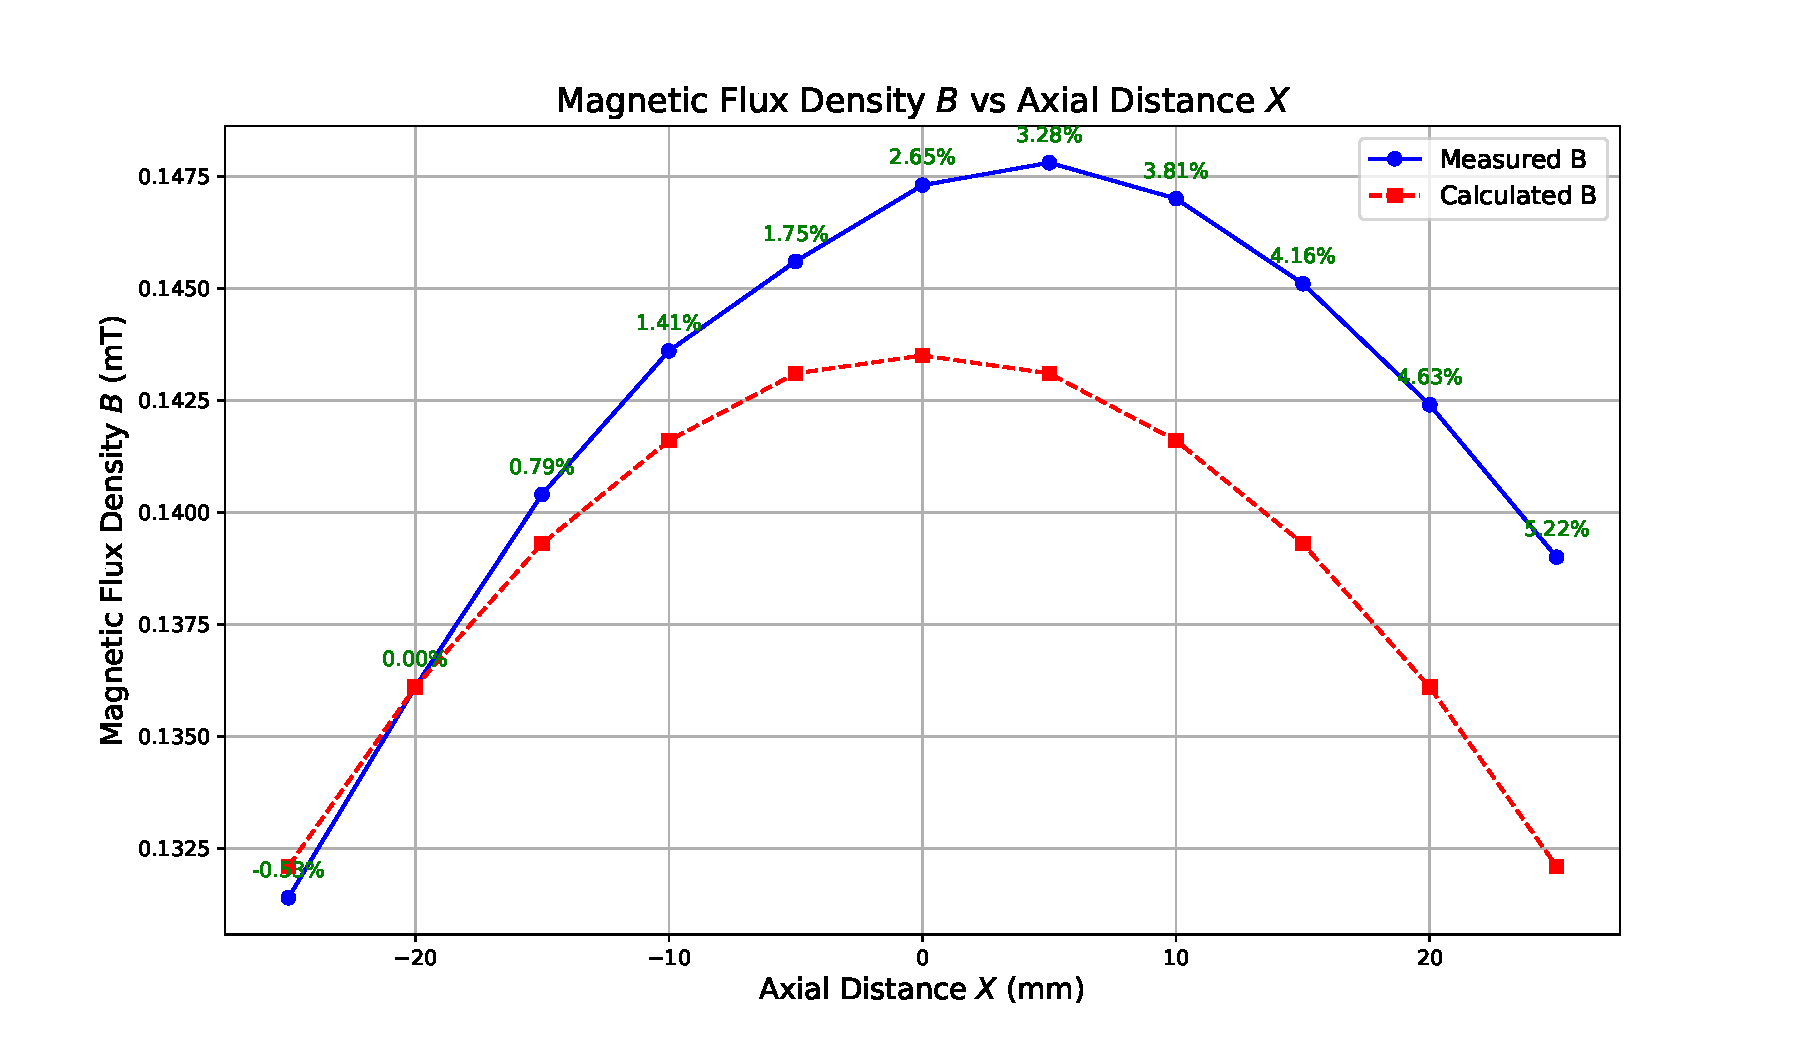
\includegraphics[width=0.6\textwidth]{./circular_current_loop_axis_magnetic_field_distribution.pdf}
    \caption{圆电流线圈轴线上磁感应强度分布}
    \label{fig:circular_current_loop_axis_magnetic_field_distribution}
\end{figure}

根据图像我们可以看出，圆电流轴线上磁感应强度分布的理论值和计算值存在一定的偏差。相对误差已经在图中标出。整体误差在 5.22\% 以内。推测误差的来源可能是磁场的中心与线圈的中心不重合以及其他系统误差。

\subsubsection{亥姆霍兹线圈轴线上磁感应强度的分布测量}

按照实验要求连接设备，将励磁电流置零并清零磁感应强度，将亥姆霍兹线圈的两个线圈串联后接入磁感应强度测试仪的励磁电流两端，调节频率电位器使频率表读数为 120 Hz，调节电流调节电位器使励磁电流有效值为 60 mA，以亥姆霍兹线圈中心为坐标原点，每隔 5 mm 测量磁感应强度的 $ U_{\text{max}} $ 值，测量过程中保持励磁电流值不变，最终将数据记录于表\ref{tab:helmholtz_coil_axis_magnetic_field_distribution}。

\begin{table}[H]
    \centering
    \renewcommand{\arraystretch}{1.2} % 调整行间距
    \begin{tabular}{|>{\centering\arraybackslash}p{2.5cm}|>{\centering\arraybackslash}p{1cm}|>{\centering\arraybackslash}p{1cm}|>{\centering\arraybackslash}p{1cm}|>{\centering\arraybackslash}p{1cm}|>{\centering\arraybackslash}p{1cm}|>{\centering\arraybackslash}p{1cm}|>{\centering\arraybackslash}p{1cm}|>{\centering\arraybackslash}p{1cm}|>{\centering\arraybackslash}p{1cm}|>{\centering\arraybackslash}p{1cm}|>{\centering\arraybackslash}p{1cm}|}
        \hline
        轴向距离 X/(mm) & -25 & -20 & -15 & -10 & -5 & 0 & 5 & 10 & 15 & 20 & 25 \\ \hline
        $U_{max}$/mV & 8.63 & 8.65 & 8.66 & 8.66 & 8.66 & 8.66 & 8.66 & 8.66 & 8.66 & 8.65 & 8.65 \\ \hline
        测量值 B/(mT) & 0.2104 & 0.2109 & 0.2112 & 0.2112 & 0.2112 & 0.2112 & 0.2112 & 0.2112 & 0.2112 & 0.2109 & 0.2109 \\ \hline
        参数 & f & I & $N_0$ & R & & & & & & & \\ \hline
        值 & 120Hz & 60mA & 400 & 105mm & & & & & & & \\ \hline
    \end{tabular}
    \caption{亥姆霍兹线圈轴线上磁场分布测量数据记录}
    \label{tab:helmholtz_coil_axis_magnetic_field_distribution}
\end{table}

根据表\ref{tab:helmholtz_coil_axis_magnetic_field_distribution}中的数据绘制磁感应强度分布曲线，如图\ref{fig:helmholtz_coil_axis_magnetic_field_distribution}所示。

\begin{figure}[H]
    \centering
    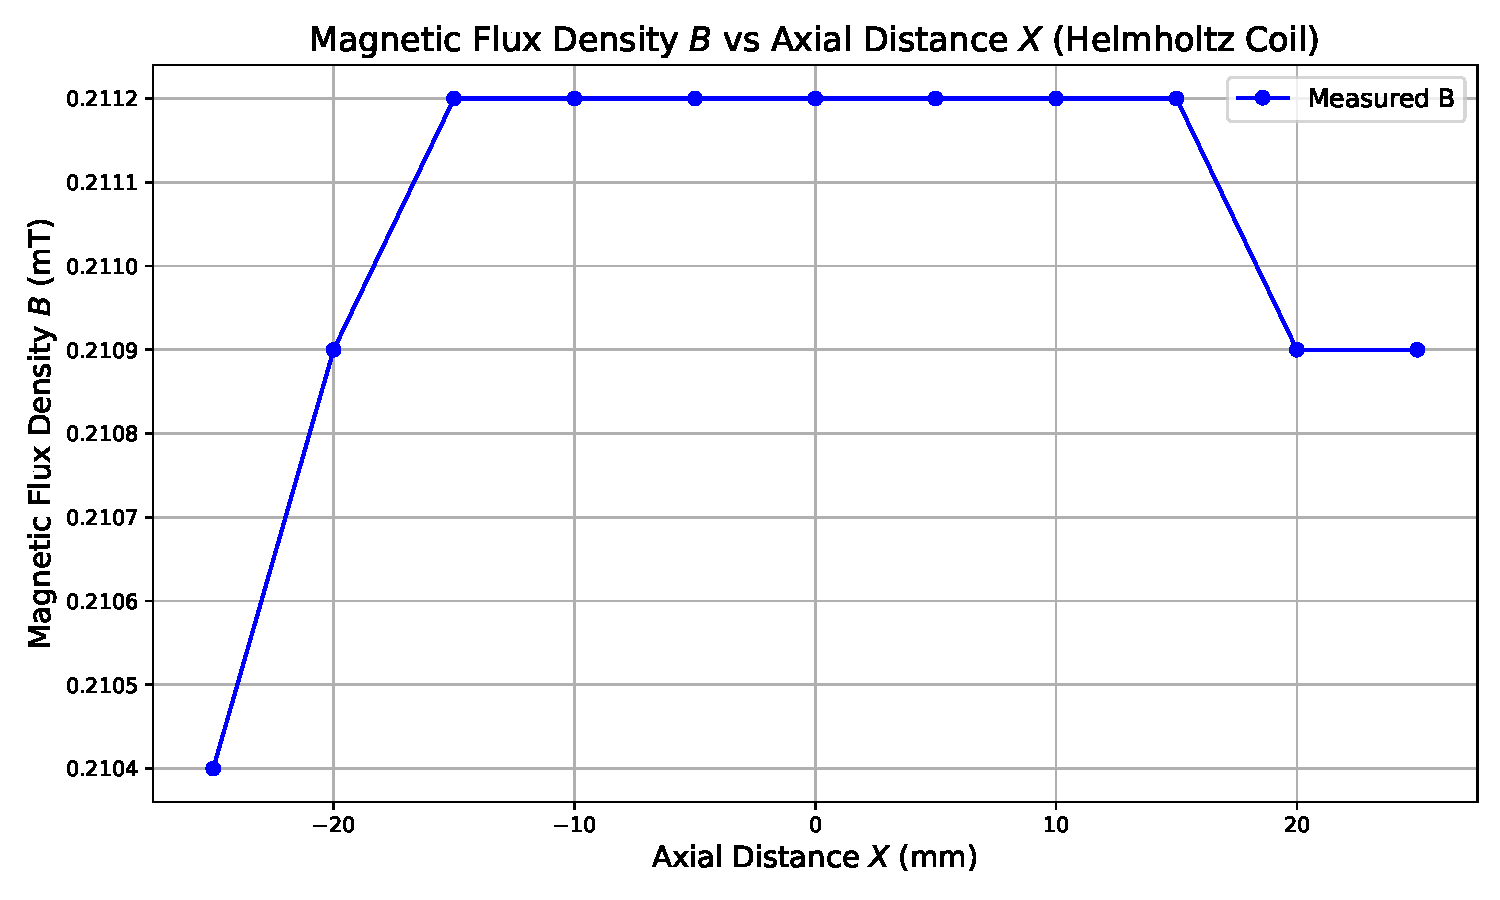
\includegraphics[width=0.6\textwidth]{./helmholtz_coil_axis_magnetic_field_distribution.pdf}
    \caption{亥姆霍兹线圈轴线上磁感应强度分布}
    \label{fig:helmholtz_coil_axis_magnetic_field_distribution}
\end{figure}

根据图像我们可以看出，亥姆霍兹线圈的磁感应强度沿轴向在中心点附近呈现比较均匀的分布，说明亥姆霍兹线圈内部的磁场可以视为是均匀的

\subsubsection{亥姆霍兹线圈沿径向磁感应强度的分布测量}

固定探测线圈的法线方向与圆电流轴线 $ D $ 的夹角为 $ 0^\circ $，通过转动探测线圈的径向移动手轮，每隔 5 mm 测量一个磁感应强度数据，沿正负径向方向测量至边缘，记录数据并绘制磁感应强度分布曲线，数据记录于表\ref{tab:helmholtz_coil_radial_magnetic_field_distribution}。


\begin{table}[H]
    \centering
    \renewcommand{\arraystretch}{1.2} % 调整行间距
    \begin{tabular}{|>{\centering\arraybackslash}p{2.5cm}|>{\centering\arraybackslash}p{1cm}|>{\centering\arraybackslash}p{1cm}|>{\centering\arraybackslash}p{1cm}|>{\centering\arraybackslash}p{1cm}|>{\centering\arraybackslash}p{1cm}|>{\centering\arraybackslash}p{1cm}|>{\centering\arraybackslash}p{1cm}|>{\centering\arraybackslash}p{1cm}|>{\centering\arraybackslash}p{1cm}|>{\centering\arraybackslash}p{1cm}|>{\centering\arraybackslash}p{1cm}|}
        \hline
        径向距离 X/(mm) & -25 & -20 & -15 & -10 & -5 & 0 & 5 & 10 & 15 & 20 & 25 \\ \hline
        $U_{max}$/mV & 8.66 & 8.66 & 8.67 & 8.67 & 8.67 & 8.67 & 8.67 & 8.66 & 8.66 & 8.65 & 8.63 \\ \hline
        测量值 B/(mT) & 0.2112 & 0.2112 & 0.2114 & 0.2114 & 0.2114 & 0.2114 & 0.2114 & 0.2112 & 0.2112 & 0.2109 & 0.2104 \\ \hline
        参数 & f & I & $N_0$ & R & & & & & & & \\ \hline
        值 & 120Hz & 60mA & 400 & 105mm & & & & & & & \\ \hline
    \end{tabular}
    \caption{亥姆霍兹线圈径向上磁场分布测量数据记录}
    \label{tab:helmholtz_coil_radial_magnetic_field_distribution}
\end{table}

根据表\ref{tab:helmholtz_coil_radial_magnetic_field_distribution}中的数据绘制磁感应强度分布曲线，如图\ref{fig:helmholtz_coil_radial_magnetic_field_distribution}所示。

\begin{figure}[H]
    \centering
    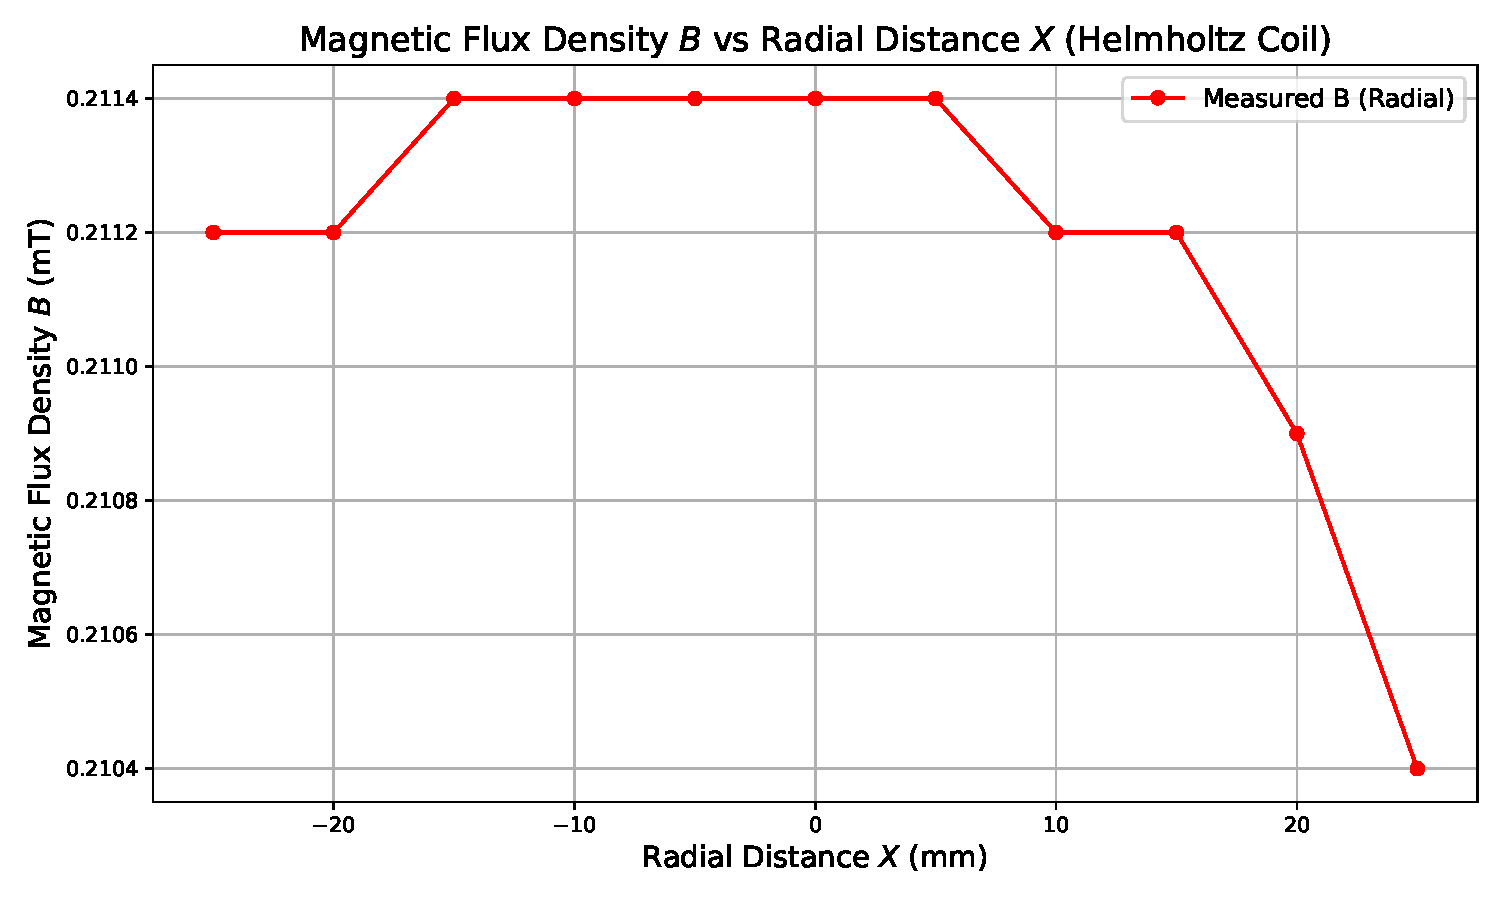
\includegraphics[width=0.6\textwidth]{./helmholtz_coil_radial_magnetic_field_distribution.pdf}
    \caption{亥姆霍兹线圈径向上磁感应强度分布}
    \label{fig:helmholtz_coil_radial_magnetic_field_distribution}
\end{figure}

根据图像我们可以看出，亥姆霍兹线圈的磁感应强度沿径向在中心点附近呈现比较均匀的分布，但在边缘附近有较为明显的衰减，这与理论计算的结果相符。

\subsubsection{验证公式$e_m = NS \omega B_m \cos \theta$}

根据实验要求，验证公式：
$$
e_m = NS \omega B_m \cos \theta
$$
其中，$ e_m $ 为感应电动势的幅值，$ N $ 为探测线圈的匝数，$ S $ 为线圈的截面积，$ \omega $ 为角频率，$ B_m $ 为磁感应强度的峰值，$ \theta $ 为探测线圈法线与磁感应强度方向的夹角。

将探测线圈固定在轴线某一位置，使探测线圈法线方向与圆电流轴线 $ D $ 的夹角从 $ 0^\circ $ 开始，逐步转动至 $ 90^\circ $、$ 180^\circ $、$ 270^\circ $，再回到 $ 0^\circ $，每改变 $ 10^\circ $ 测量一组感应电压数据，探测线圈转角与感应电压数据记录于表\ref{tab:probe_coil_angle_induced_voltage_data}。


\begin{table}[H]
\centering
\begin{tabular}{|c|c|c|c|c|c|c|c|c|c|c|}
\hline
探测线圈转角θ & 0 & 10 & 20 & 30 & 40 & 50 & 60 & 70 & 80 & 90\\ 
\hline
U (mV) & 8.68 & 8.52 & 8.17 & 7.56 & 6.75 & 5.72 & 4.49 & 3.11 & 1.61 & 0.11\\
\hline
计算值：$U = U_{max}\cos θ$ & 8.68 & 8.55 & 8.16 & 7.52 & 6.65 & 5.58 & 4.34 & 2.97 & 1.51 & 0.00\\
\hline
误差 (\%) & 0.00 & 0.04 & 0.02 & 0.08 & 0.23 & 0.45 & 0.79 & 1.53 & 4.35 & -\\
\hline
探测线圈转角θ & 100 & 110 & 120 & 130 & 140 & 150 & 160 & 170 & 180 & 190\\
\hline
U (mV) & 1.37 & 2.90 & 4.31 & 5.56 & 6.62 & 7.52 & 8.17 & 8.54 & 8.62 & 8.43\\
\hline
计算值：$U = U_{max}\cos θ$ & 1.51 & 2.97 & 4.34 & 5.58 & 6.65 & 7.52 & 8.16 & 8.55 & 8.68 & 8.55\\
\hline
误差 (\%) & 9.08 & 2.30 & 0.68 & 0.34 & 0.43 & 0.04 & 0.17 & 0.09 & 0.69 & 1.38\\
\hline
探测线圈转角θ & 200 & 210 & 220 & 230 & 240 & 250 & 260 & 270 & 280 & 290\\
\hline
U (mV) & 8.04 & 7.31 & 6.42 & 5.34 & 3.86 & 2.55 & 0.94 & 0.54 & 1.98 & 3.38\\
\hline
计算值：$U = U_{max}\cos θ$ & 8.16 & 7.52 & 6.65 & 5.58 & 4.34 & 2.97 & 1.51 & 0.00 & 1.51 & 2.97\\
\hline
误差 (\%) & 1.43 & 2.76 & 3.46 & 4.30 & 11.08 & 14.14 & 37.68 & - & 3.15 & 1.39\\
\hline
探测线圈转角θ & 300 & 310 & 320 & 330 & 340 & 350 & 360 & & & \\
\hline
U (mV) & 4.69 & 5.81 & 6.78 & 7.68 & 8.24 & 8.59 & 8.67 & & & \\
\hline
计算值：$U = U_{max}\cos θ$ & 4.34 & 5.58 & 6.65 & 7.52 & 8.16 & 8.55 & 8.68 & & &\\
\hline
误差 (\%) & 8.09 & 4.15 & 1.98 & 2.18 & 1.03 & 0.49 & 0.12 & & & \\
\hline
\end{tabular}
\caption{探测线圈转角与感应电压数据记录}
\label{tab:probe_coil_angle_induced_voltage_data}
\end{table}

根据表\ref{tab:probe_coil_angle_induced_voltage_data}中的数据绘制探测线圈转角与感应电压的关系曲线，如图\ref{fig:probe_coil_angle_induced_voltage}所示。

\begin{figure}[H]
    \centering
    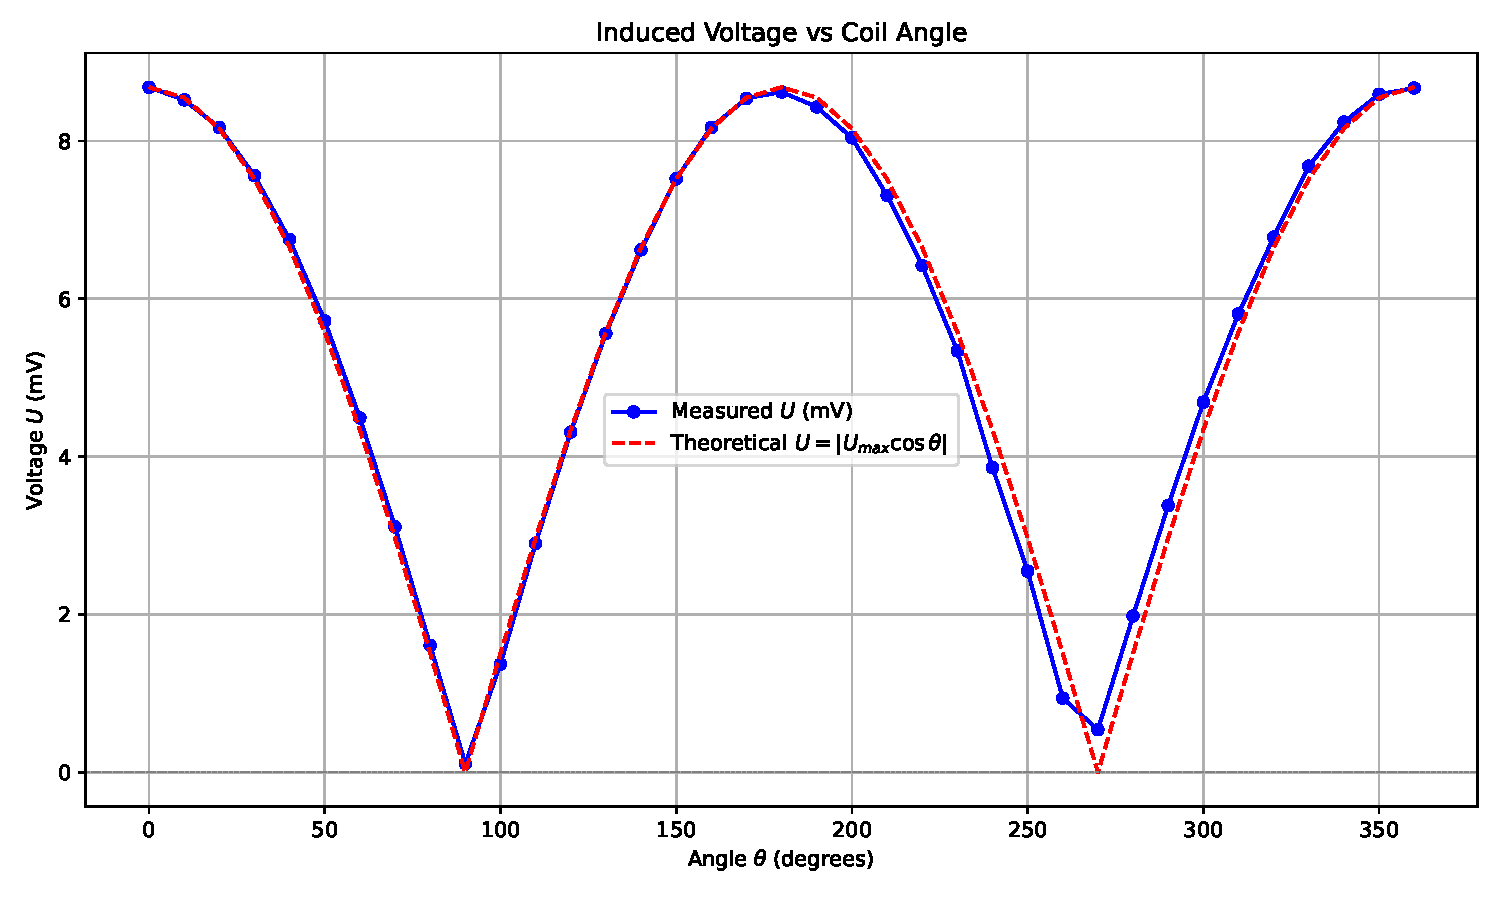
\includegraphics[width=0.6\textwidth]{./probe_coil_angle_induced_voltage.pdf}
    \caption{探测线圈转角与感应电压关系}
    \label{fig:probe_coil_angle_induced_voltage}
\end{figure}

由图可见，测量值与计算值曲线基本吻合，验证了公式 $ e_m = NS \omega B_m \cos \theta $ 的正确性。

\subsubsection{励磁电流大小对磁感应强度的影响}

将探测线圈固定在亥姆霍兹线圈中心点，确保其法线方向与圆电流轴线 $ D $ 的夹角为 $ 0^\circ $ 并保持不变。调节磁感应强度测试仪输出电流频率，在 $ 20 \, \text{Hz} \sim 150 \, \text{Hz} $ 范围内，每次改变 $ 10 \, \text{Hz} $，测量并记录每次频率变化对应的感应电动势值，记录数据于表\ref{tab:magnetic_field_data}。

\begin{table}[H]
\centering
\begin{tabular}{|c|>{\centering\arraybackslash}p{1cm}|>{\centering\arraybackslash}p{1cm}|>{\centering\arraybackslash}p{1cm}|>{\centering\arraybackslash}p{1cm}|>{\centering\arraybackslash}p{1cm}|>{\centering\arraybackslash}p{1cm}|>{\centering\arraybackslash}p{1cm}|>{\centering\arraybackslash}p{1cm}|>{\centering\arraybackslash}p{1cm}|>{\centering\arraybackslash}p{1cm}|>{\centering\arraybackslash}p{1cm}|}
\hline
频率 f (Hz) & 20 & 30 & 40 & 50 & 60 & 70 & 80 & 90 & 100 & 110 & 120\\ 
\hline
$U_{max}$ (mV) & 1.45 & 2.16 & 2.89 & 3.61 & 4.33 & 5.05 & 5.76 & 6.48 & 7.21 & 7.94 & 8.66\\
\hline
测量值 (mT) & 0.2121 & 0.2107 & 0.2114 & 0.2113 & 0.2112 & 0.2111 & 0.2107 & 0.2107 & 0.2110 & 0.2112 & 0.2112\\
\hline
\end{tabular}
\caption{励磁电流频率与最大感应电压及磁感应强度数据记录}
\label{tab:magnetic_field_data}
\end{table}

根据表\ref{tab:magnetic_field_data}中的数据绘制励磁电流频率与磁感应强度的关系曲线，如图\ref{fig:magnetic_field}所示。

\begin{figure}[H]
    \centering
    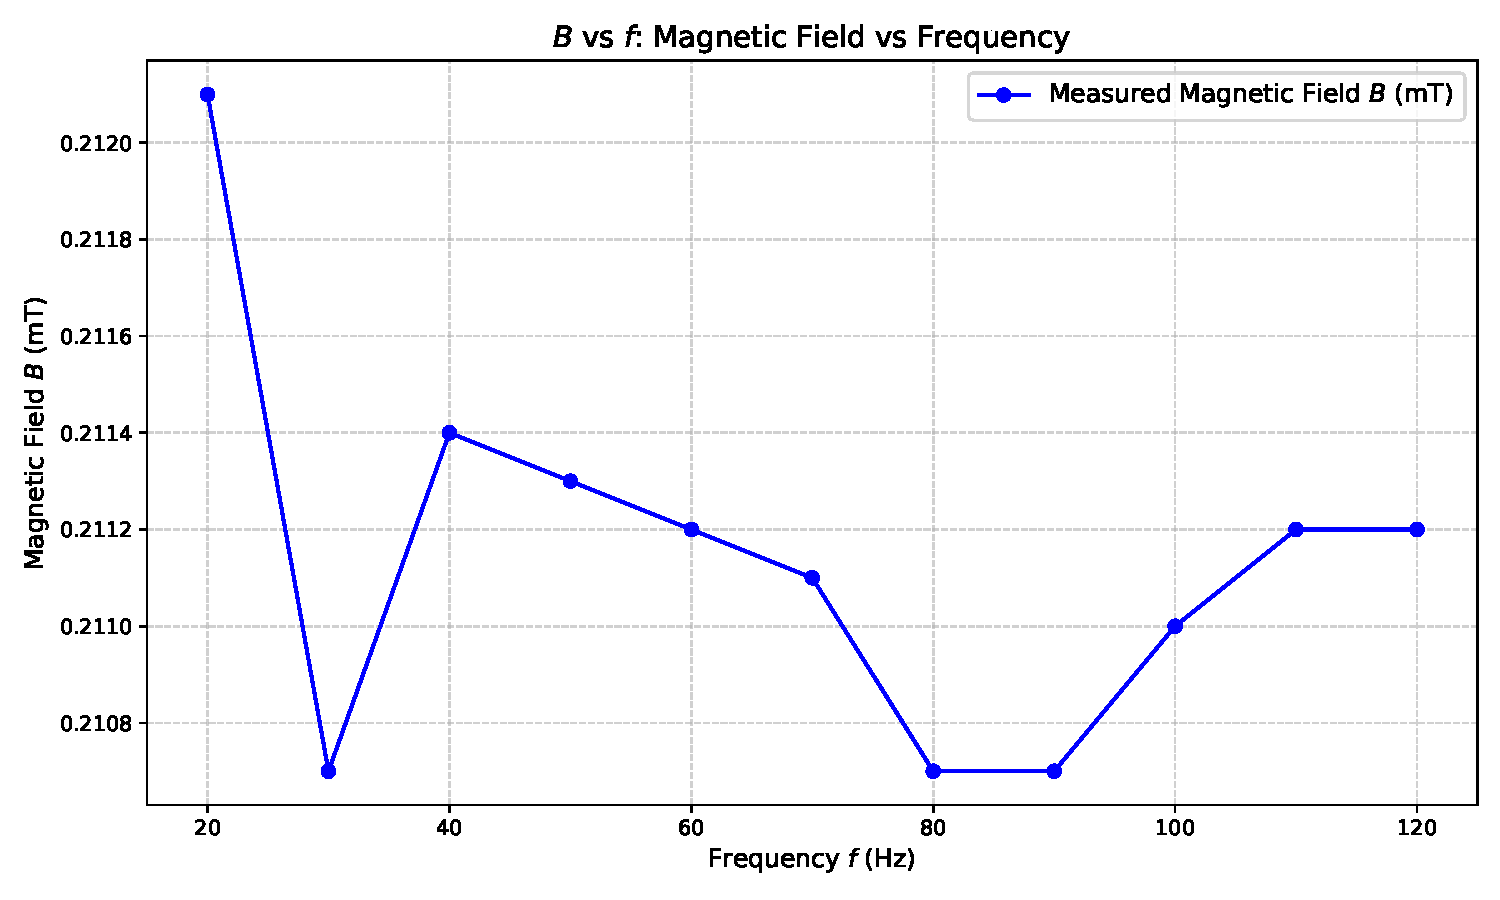
\includegraphics[width=0.6\textwidth]{./magnetic_field.pdf}
    \caption{励磁电流频率与磁感应强度关系}
    \label{fig:magnetic_field}
\end{figure}

根据图片可以看出，磁感应强度随着励磁电流频率的变化而变化，但这一变化几乎不呈现规律性，并且总体的偏差在7\%以内。注意到本组数据内部相差很小，在作图时纵轴的分度值也很小，因此可以认为励磁电流的频率对磁感应强度的大小并没有影响。这和理论预期相吻合。

\section{总结与思考}

\subsection{实验中遇到的问题}
\begin{enumerate}
    \item 实验中，由于温度的变化可能会对霍尔元件的性能造成影响，因此可能导致霍尔元件灵敏度的测定出现偏差。
    \item 在验证公式。$e_m = NS \omega B_m \cos \theta$时，探测线圈在旋转时比较费力，可能会出现旋转的角度不够精确的情况，为实验带来误差。
    \item 在验证公式。$e_m = NS \omega B_m \cos \theta$时，零度处和一百八十度处在理论上都应当取极大值，但事实上这两个测量结果并不相同。推测实验装置存在一定的系统误差。
\end{enumerate}

\subsection{实验的改进方法}
\begin{enumerate}
    \item 在实验中，可以在实验室内部保持一个恒定的温度，避免温度变化对霍尔元件性能的影响。也可以在不同的温度条件下进行试验，验证温度对霍尔元件性能的影响是否会对实验造成较大误差。
    \item 上一个问题也可以从理论推导的角度进行解决。
      霍尔电压 \( V_H \) 与霍尔系数 \( R_H \)、驱动电流 \( I_S \)、磁感应强度 \( B \) 和厚度 \( d \) 的关系为：
        \[
        V_H = \frac{R_H \cdot I_S \cdot B}{d}
        \]
        其中：
        \[
        R_H = \frac{1}{n \cdot q}
        \]
        温度变化通过改变载流子浓度 \( n \) 和迁移率 \( \mu \)，影响霍尔系数 \( R_H \)，从而改变霍尔电压 \( V_H \)。
        例如，载流子迁移率 \( \mu \) 通常随温度变化，满足如下经验公式：
        \[
        \mu(T) \propto T^{-\gamma}
        \]
        其中 \( \gamma \) 是与材料特性相关的指数，通常在 \( 1.5 \sim 2.5 \) 之间。迁移率降低会减少霍尔系数 \( R_H \)，从而降低霍尔电压 \( V_H \)。

        因此，我们可以通过查阅相关公式，通过考虑 \( R_H \)、\( I_S \) 和 \( d \) 随温度的变化，得到修正公式
                \[
        V_H(T) = \frac{R_H(T) \cdot I_S(T) \cdot B}{d}
        \]
        来减少温度带来的误差对实验结果的影响。

    \item 在验证公式。$e_m = NS \omega B_m \cos \theta$时，可以适当松动探测线圈的固定装置，使之更易于旋转。
    \item 在验证公式。$e_m = NS \omega B_m \cos \theta$时，零度和一百八十度处测得的电压值不同，这可能是由于做实验的环境下地磁场不能忽略。通过查阅资料，知道中纬度地区的地磁场强度大致为0.02-0.06 mT。这样的大小已经足以为本实验造成误差。因此，若要更精确的完成实验，应当使用不同的仪器，在不同的地点，以不同的取向反复进行测量以减小地磁场的影响。
\end{enumerate}

\subsection{思考题}

\begin{enumerate}
  \item \textbf{为什么准备工作中需要我们在仪器使用前开机预热10分钟？} \\
    首先，我们在读取数据前需要励磁电流达到稳定，而仪器预热能够使电流更稳定，满足实验要求。其次，因为仪器在运行时会产生一定的热量，如果仪器在使用前没有预热，可能会导致仪器在运行时温度不稳定。在前文中我们讨论到，温度会影响霍尔元件的性能。如果没有经过预热，那么在实验过程中霍尔元件可能会存在不断升温的情况，这样会为实验引入一个不断变化的系统误差，难以进行数据处理。
  \item \textbf{如果在攻击波前开一磁场空洞，能否将地球移动？} \\
    我认为可以。太阳风中的带电粒子接近地球时，受到地球磁场的作用而被偏转和排斥。根据力相互作用的规律，可以推断太阳风对地球产生斥力。也就是说，这一斥力和万有引力等力一起构成地球自转的向心力。当这一排斥力消失时，地球收到的引力将会增大，这将导致地球向太阳的轨道半径缩小，使地球向太阳靠近。
  \item \textbf{分析本实验主要误差来源，计算磁感应强度B的合成不确定度（分别取$I_M$=0.3A，$I_H$=2mA)}
    \begin{itemize}
      \item \textbf{主要误差来源}：
      \begin{enumerate}
        \item 仪器误差：磁感应强度测试仪的误差和精确度不足。
        \item 环境误差：地磁场对实验的影响，温度对霍尔元件性能的影响。
        \item 人为误差：实验者在操作过程中的误差，例如旋转探测线圈角度不精准等对实验造成误差。
        \item 系统误差：通过对称测量法无法消除的爱廷豪森效应带来的误差。
      \end{enumerate}
      \item \textbf{合成不确定度}：
      \begin{enumerate}
        \item 根据公式$$B = \frac{U_H}{K_H \cdot I_H}$$可以知道
          \[
\mu(B) = \sqrt{\left(\frac{\mu(U_H)}{U_H}\right)^2 + \left(\frac{\mu(K_H)}{K_H}\right)^2 + \left(\frac{\mu(I_H)}{I_H}\right)^2}
\]
可以计算出磁感应强度的合成不确定度$\mu(B) = 0.5 \, \text{mT}$
      \end{enumerate}
    \end{itemize}
\end{enumerate}

\section{原始数据记录表}
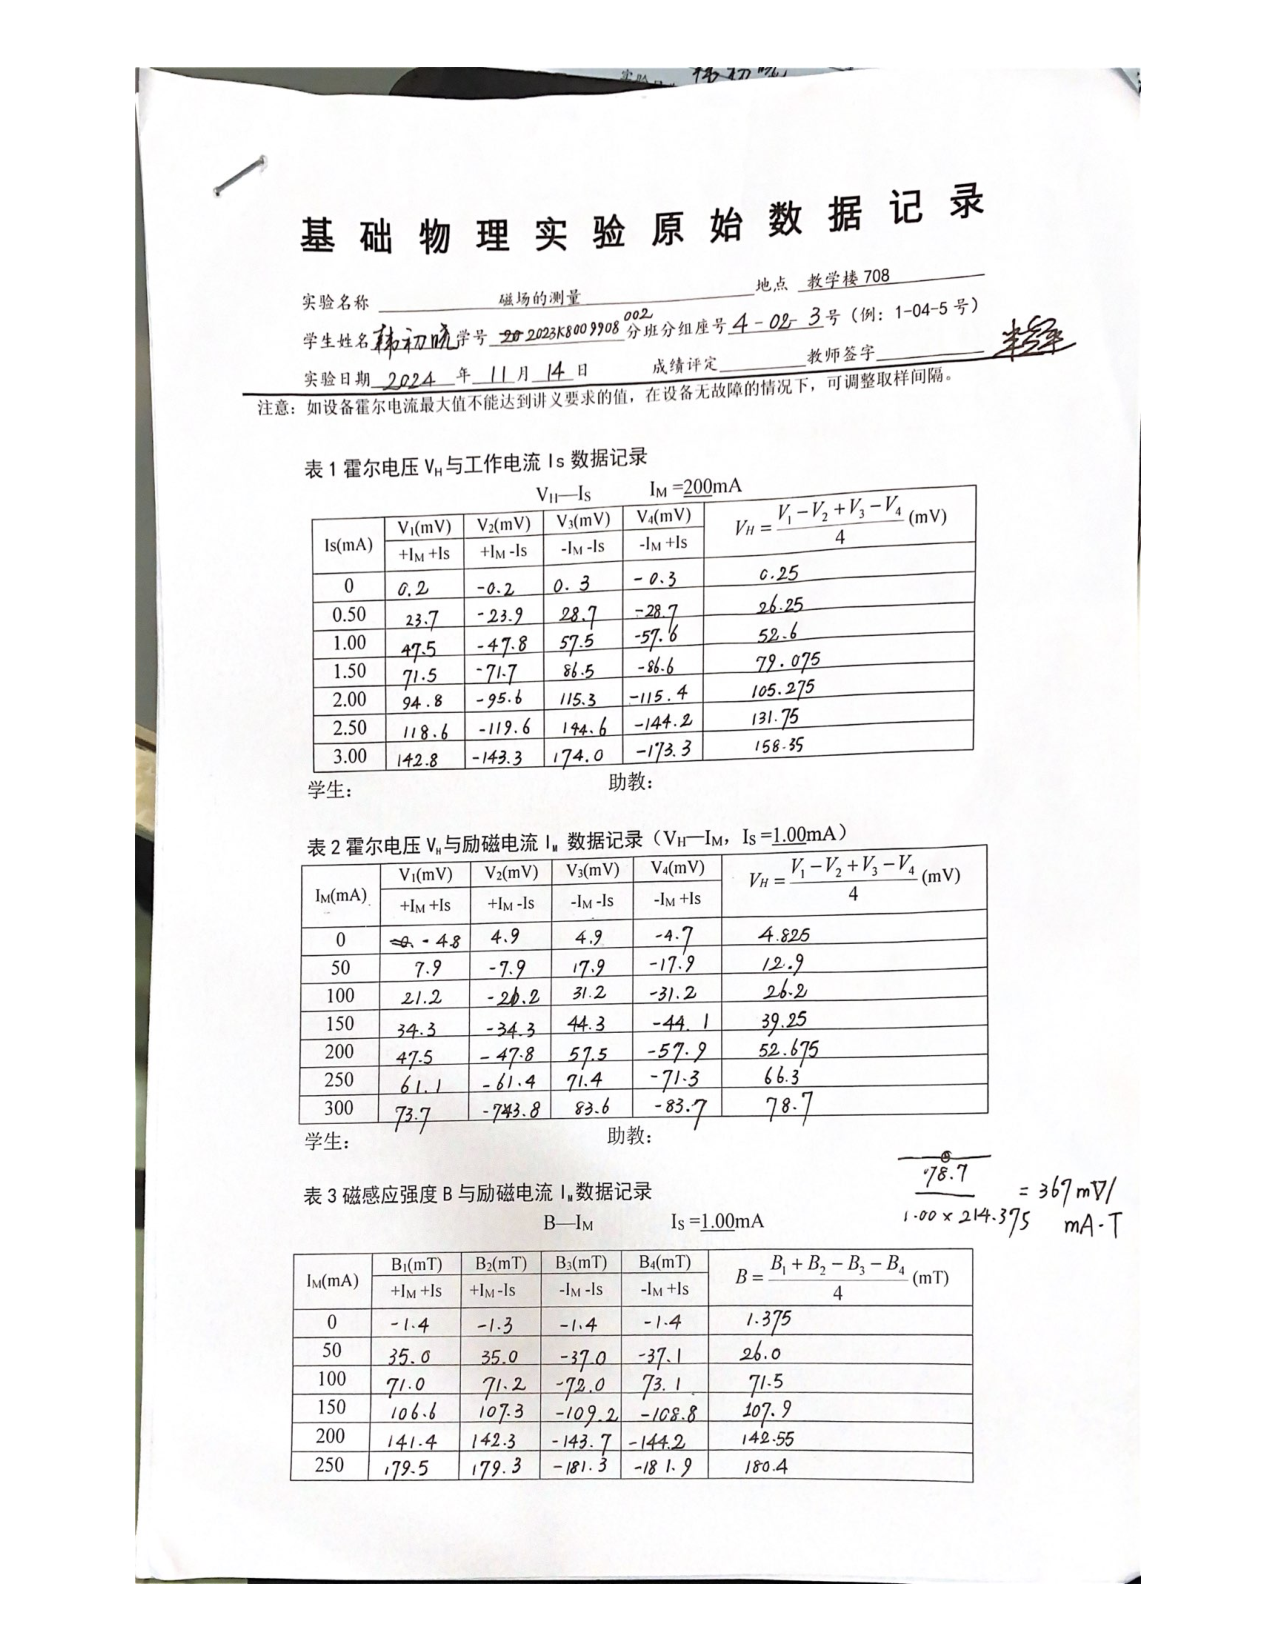
\includepdf[pages=-]{./韩初晓-磁场的测量-数据.pdf}

\end{document}

% VScode 常用快捷键：

% F2:                       变量重命名
% Ctrl + Enter:             行中换行
% Alt + up/down:            上下移行
% 鼠标中键 + 移动:           快速多光标
% Shift + Alt + up/down:    上下复制
% Ctrl + left/right:        左右跳单词
% Ctrl + Backspace/Delete:  左右删单词    
% Shift + Delete:           删除此行
% Ctrl + J:                 打开 VScode 下栏(输出栏)
% Ctrl + B:                 打开 VScode 左栏(目录栏)
% Ctrl + `:                 打开 VScode 终端栏
% Ctrl + 0:                 定位文件
% Ctrl + Tab:               切换已打开的文件(切标签)
% Ctrl + Shift + P:         打开全局命令(设置)

% Latex 常用快捷键：

% Ctrl + Alt + J:           由代码定位到PDF


